% !TeX program = xelatex
% 本文件按所给旧版 cctbook 模板的版式参数等效重建。
% 正文中的 MathType 7 公式采用原稿导出的高分辨率透明图，以避免公式内容损失。
\documentclass[12pt,oneside,openany,fontset=windows]{ctexbook}
\usepackage{amsmath,amssymb}
\usepackage{graphicx}
\usepackage{fancyhdr}
\usepackage{geometry}
\usepackage{titlesec}
\usepackage{setspace}
\usepackage{color}

\geometry{
  a4paper,
  left=29.62mm,
  top=34.92mm,
  textwidth=15.3cm,
  textheight=22.6cm,
  headsep=0.5cm,
  footskip=29.02pt
}
\setmainfont{Times New Roman}
\setlength{\parindent}{2em}
\setlength{\parskip}{0pt}
\setstretch{1.667}
\setlength{\emergencystretch}{3em}
\allowdisplaybreaks[4]
\graphicspath{{assets/formulas/}}

\ctexset{
  chapter = {
    name = {第,章},
    number = \chinese{chapter},
    format = \centering\heiti\zihao{3},
    nameformat = \heiti\zihao{3},
    titleformat = \heiti\zihao{3},
    aftername = \quad,
    beforeskip = -22pt,
    afterskip = 15pt,
    pagestyle = thesis
  }
}
\renewcommand{\contentsname}{目\quad 录}
\renewcommand{\bibname}{参考文献}
\numberwithin{equation}{section}

\fancypagestyle{thesis}{
  \fancyhf{}
  \renewcommand{\headrulewidth}{0pt}
  \cfoot{\thepage}
}

\begin{document}
\begin{titlepage}
\vspace*{1cm} \LARGE\heiti\vspace*{-16.5pt}
\begin{center}
{\heiti\zihao{2} $(L,M)$-模糊粗结构}
\end{center}
\vspace*{2mm}\songti

\begin{center}
{\Large\zihao{4} 赵子函}
\end{center}

\Large\vspace*{0mm}
\begin{center}
(\zihao{4}安徽师范大学数学与统计学院, 安徽, 芜湖, 241000)
\end{center}\vspace{6mm}
\vfill\large\baselineskip=31pt
\begin{center}
{\zihao{4}安徽师范大学硕士学位论文}
\end{center}
\vspace*{-25.4pt}
\begin{center}
{\zihao{4}二零二六年八月}
\end{center}
\end{titlepage}

\newpage
\pagestyle{plain}
\pagenumbering{Roman}
\chapter*{}
\addcontentsline{toc}{chapter}{摘要}
\begin{center}
{\heiti\zihao{3} $(L,M)$-模糊粗结构}
\end{center}
\begin{center}
\vspace{-0.13cm} {\zihao{4}\heiti 摘\quad\quad 要}\\
\end{center}
\baselineskip=24pt
{\zihao{-4}

基于完全分配格\hspace{0pt}\penalty0\raisebox{-2pt}{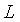
\includegraphics[width=10pt,height=11pt]{assets/formulas/formula-0002.png}}\penalty0\hspace{0pt}和\hspace{0pt}\penalty0\raisebox{-2pt}{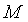
\includegraphics[width=13.95pt,height=11pt]{assets/formulas/formula-0003.png}}\penalty0\hspace{0pt}, 我们提出了一种格值粗结构的新方法. 首先,我们引入了\hspace{0pt}\penalty0\raisebox{-4pt}{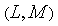
\includegraphics[width=29pt,height=13pt]{assets/formulas/formula-0004.png}}\penalty0\hspace{0pt}-模糊熵、\hspace{0pt}\penalty0\raisebox{-4pt}{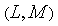
\includegraphics[width=29pt,height=13pt]{assets/formulas/formula-0005.png}}\penalty0\hspace{0pt}-模糊拟粗结构、\hspace{0pt}\penalty0\raisebox{-4pt}{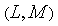
\includegraphics[width=29pt,height=13pt]{assets/formulas/formula-0006.png}}\penalty0\hspace{0pt}-模糊半粗结构的概念,并研究了\hspace{0pt}\penalty0\raisebox{-4pt}{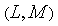
\includegraphics[width=29pt,height=13pt]{assets/formulas/formula-0007.png}}\penalty0\hspace{0pt}-模糊粗空间之间的映射性质. 其次, 我们从\hspace{0pt}\penalty0\raisebox{-4pt}{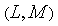
\includegraphics[width=29pt,height=13pt]{assets/formulas/formula-0008.png}}\penalty0\hspace{0pt}-模糊关系等方面出发, 构造了典型的\hspace{0pt}\penalty0\raisebox{-4pt}{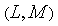
\includegraphics[width=29pt,height=13pt]{assets/formulas/formula-0009.png}}\penalty0\hspace{0pt}-模糊粗结构实例. 最后, 我们引入了\hspace{0pt}\penalty0\raisebox{-4pt}{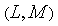
\includegraphics[width=29pt,height=13pt]{assets/formulas/formula-0010.png}}\penalty0\hspace{0pt}-模糊球结构的概念, 并用其刻画\hspace{0pt}\penalty0\raisebox{-4pt}{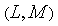
\includegraphics[width=29pt,height=13pt]{assets/formulas/formula-0011.png}}\penalty0\hspace{0pt}-模糊粗结构.

\vspace{0.5cm} {\heiti\zihao{4}关键词:}\,
\hspace{0pt}\penalty0\raisebox{-4pt}{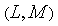
\includegraphics[width=29pt,height=13pt]{assets/formulas/formula-0012.png}}\penalty0\hspace{0pt}-模糊粗结构；\hspace{0pt}\penalty0\raisebox{-4pt}{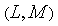
\includegraphics[width=29pt,height=13pt]{assets/formulas/formula-0013.png}}\penalty0\hspace{0pt}-模糊粗空间；\hspace{0pt}\penalty0\raisebox{-4pt}{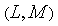
\includegraphics[width=29pt,height=13pt]{assets/formulas/formula-0014.png}}\penalty0\hspace{0pt}-模糊关系；\hspace{0pt}\penalty0\raisebox{-4pt}{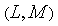
\includegraphics[width=29pt,height=13pt]{assets/formulas/formula-0015.png}}\penalty0\hspace{0pt}-模糊球结构
}

\newpage
\chapter*{}
\addcontentsline{toc}{chapter}{Abstract}
\vspace*{9.9pt}
\begin{center}
\vspace{0.3cm}{\Large\bfseries $(L,M)$-Fuzzy Coarse Structure}
\end{center}
\vspace*{4.2pt}
\begin{center}
\vspace{0.2cm} {\large\bfseries Abstract}
\end{center}
\vspace*{-6.4pt}
\zihao{-4}

Based on completely distributive lattices \hspace{0pt}\penalty0\raisebox{0pt}{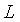
\includegraphics[width=10pt,height=11pt]{assets/formulas/formula-0565.png}}\penalty0\hspace{0pt} and \hspace{0pt}\penalty0\raisebox{0pt}{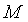
\includegraphics[width=13.95pt,height=11pt]{assets/formulas/formula-0566.png}}\penalty0\hspace{0pt}, we propose a novel approach to lattice-valued coarse structures. First, we introduce the concepts of \hspace{0pt}\penalty0\raisebox{0pt}{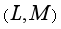
\includegraphics[width=30.25pt,height=14.3pt]{assets/formulas/formula-0567.png}}\penalty0\hspace{0pt}-fuzzy entourage, \hspace{0pt}\penalty0\raisebox{0pt}{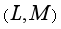
\includegraphics[width=30.25pt,height=14.3pt]{assets/formulas/formula-0568.png}}\penalty0\hspace{0pt}-fuzzy quasi coarse structures, and\hspace{0pt}\penalty0\raisebox{0pt}{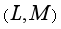
\includegraphics[width=30.25pt,height=14.3pt]{assets/formulas/formula-0569.png}}\penalty0\hspace{0pt}-fuzzy semi coarse structures, and investigate mapping properties between \hspace{0pt}\penalty0\raisebox{0pt}{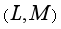
\includegraphics[width=30.25pt,height=14.3pt]{assets/formulas/formula-0570.png}}\penalty0\hspace{0pt}-fuzzy coarse spaces. Second, we construct canonical example of \hspace{0pt}\penalty0\raisebox{0pt}{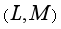
\includegraphics[width=30.25pt,height=14.3pt]{assets/formulas/formula-0571.png}}\penalty0\hspace{0pt}-fuzzy coarse structures from perspectives such as \hspace{0pt}\penalty0\raisebox{0pt}{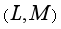
\includegraphics[width=30.25pt,height=14.3pt]{assets/formulas/formula-0572.png}}\penalty0\hspace{0pt}- fuzzy relations. Finally, we introduce the notion of \hspace{0pt}\penalty0\raisebox{0pt}{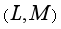
\includegraphics[width=30.25pt,height=14.3pt]{assets/formulas/formula-0573.png}}\penalty0\hspace{0pt}-fuzzy ball structures and employ them to characterize \hspace{0pt}\penalty0\raisebox{0pt}{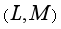
\includegraphics[width=30.25pt,height=14.3pt]{assets/formulas/formula-0574.png}}\penalty0\hspace{0pt}-fuzzy coarse structures.

\vspace{0.3cm}
{\large\bfseries Keywords:}\,
\hspace{0pt}\penalty0\raisebox{-4pt}{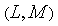
\includegraphics[width=29pt,height=13pt]{assets/formulas/formula-0575.png}}\penalty0\hspace{0pt}-fuzzy coarse structure; \hspace{0pt}\penalty0\raisebox{-4pt}{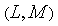
\includegraphics[width=29pt,height=13pt]{assets/formulas/formula-0576.png}}\penalty0\hspace{0pt}-fuzzy coarse space; \hspace{0pt}\penalty0\raisebox{-4pt}{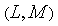
\includegraphics[width=29pt,height=13pt]{assets/formulas/formula-0577.png}}\penalty0\hspace{0pt}-fuzzy relation; \hspace{0pt}\penalty0\raisebox{-4pt}{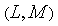
\includegraphics[width=29pt,height=13pt]{assets/formulas/formula-0578.png}}\penalty0\hspace{0pt}-fuzzy ball structure

\newpage
{\color{white}1}
\newpage

\tableofcontents
\mainmatter
\pagestyle{thesis}
\zihao{-4}
\baselineskip=24pt

\chapter{引\ \ 言}
\vspace{0.2cm}
在经典拓扑学的研究中, 研究者们长期聚焦于由拓扑定义的小尺度结构, 如邻域系统、连续性等, 度量空间中连续性的研究便是典型范例. 然而, 在定义度量空间上映射的连续性时, 度量本身蕴含的大量信息往往被忽略. 与经典拓扑学相对, 数学研究有时需关注其对偶情形, 即大尺度几何（亦称粗几何）. 粗几何这一学科现已与拓扑学、指标理论等建立了深刻联系\cite{ref1}. Roe在其专著中对粗几何进行了系统论述\cite{ref2}.

模糊集的概念由Zadeh首创, 在Zadeh的开创性论文中, 模糊集被视为一个函数\hspace{0pt}\penalty0\raisebox{-6pt}{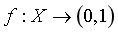
\includegraphics[width=59pt,height=17pt]{assets/formulas/formula-0016.png}}\penalty0\hspace{0pt}, 其值\hspace{0pt}\penalty0\raisebox{-6pt}{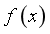
\includegraphics[width=24.95pt,height=17pt]{assets/formulas/formula-0017.png}}\penalty0\hspace{0pt}通常解释为元素\hspace{0pt}\penalty0\raisebox{-3pt}{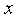
\includegraphics[width=9pt,height=10pt]{assets/formulas/formula-0018.png}}\penalty0\hspace{0pt}属于该模糊集的确定程度\cite{ref3}. 众所周知, 模糊集理论已发展成为一个极为活跃的研究领域. 尽管粗几何理论在数学的诸多分支中扮演着重要角色, 但在Zarichnyi于2009年的工作之前\cite{ref4}, 粗几何从未在模糊背景下被系统研究. 据我们所知, 迄今为止关于模糊粗结构本身的研究并不多（近期一些论文探讨了模糊度量空间中的大尺度几何性质, 但其粗结构集本身仍是经典的）. 而且, 现有的模糊粗结构研究多基于单一格\hspace{0pt}\penalty0\raisebox{-2pt}{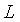
\includegraphics[width=10pt,height=11pt]{assets/formulas/formula-0019.png}}\penalty0\hspace{0pt}, 这种单格框架在处理某些复杂的渐近行为或需要同时刻画不同层次的不确定性时可能会不够合适\cite{ref5}. 为更精细、更灵活地描述大尺度模糊结构, 亟需引入双格框架.

受严从华和王永超对粗结构模糊化工作的启发\cite{ref6}, 本文将引入\hspace{0pt}\penalty0\raisebox{-4pt}{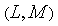
\includegraphics[width=29pt,height=13pt]{assets/formulas/formula-0020.png}}\penalty0\hspace{0pt}-模糊粗结构的概念, 并给出其等价刻画. 本文的结构如下：在第二节中, 我们列出一些完全分配格、模糊关系、单格模糊粗结构的基本概念与结果. 在第三节中, 我们给出\hspace{0pt}\penalty0\raisebox{-4pt}{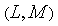
\includegraphics[width=29pt,height=13pt]{assets/formulas/formula-0021.png}}\penalty0\hspace{0pt}-模糊粗结构概念和\hspace{0pt}\penalty0\raisebox{-4pt}{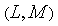
\includegraphics[width=29pt,height=13pt]{assets/formulas/formula-0022.png}}\penalty0\hspace{0pt}-模糊粗空间之间的态射, 并列举了\hspace{0pt}\penalty0\raisebox{-4pt}{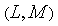
\includegraphics[width=29pt,height=13pt]{assets/formulas/formula-0023.png}}\penalty0\hspace{0pt}-模糊粗结构实例. 在第四节中, 我们引入\hspace{0pt}\penalty0\raisebox{-4pt}{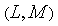
\includegraphics[width=29pt,height=13pt]{assets/formulas/formula-0024.png}}\penalty0\hspace{0pt}-模糊球结构的概念, 并建立其与\hspace{0pt}\penalty0\raisebox{-4pt}{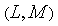
\includegraphics[width=29pt,height=13pt]{assets/formulas/formula-0025.png}}\penalty0\hspace{0pt}-模糊粗结构之间的相互刻画关系.


\chapter{预备知识}
\vspace{0.2cm}
在本文中, 称一个非空集合\hspace{0pt}\penalty0\raisebox{-2pt}{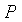
\includegraphics[width=11pt,height=11pt]{assets/formulas/formula-0026.png}}\penalty0\hspace{0pt}为一个偏序集, 如果它中的一个二元关系\hspace{0pt}\penalty0\raisebox{-2pt}{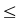
\includegraphics[width=10.5pt,height=10.5pt]{assets/formulas/formula-0027.png}}\penalty0\hspace{0pt}满足自反性、反对称性和传递性. 称\hspace{0pt}\penalty0\raisebox{-2pt}{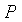
\includegraphics[width=11pt,height=11pt]{assets/formulas/formula-0028.png}}\penalty0\hspace{0pt}的子集\hspace{0pt}\penalty0\raisebox{-2pt}{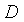
\includegraphics[width=12pt,height=11pt]{assets/formulas/formula-0029.png}}\penalty0\hspace{0pt}为有向的, 如果它是非空的, 并且\hspace{0pt}\penalty0\raisebox{-2pt}{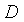
\includegraphics[width=12pt,height=11pt]{assets/formulas/formula-0030.png}}\penalty0\hspace{0pt}的每个有限子集在\hspace{0pt}\penalty0\raisebox{-2pt}{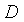
\includegraphics[width=12pt,height=11pt]{assets/formulas/formula-0031.png}}\penalty0\hspace{0pt}中都有上界\cite{ref7}.

本文中, \hspace{0pt}\penalty0\raisebox{-2pt}{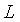
\includegraphics[width=10pt,height=11pt]{assets/formulas/formula-0032.png}}\penalty0\hspace{0pt}和\hspace{0pt}\penalty0\raisebox{-2pt}{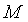
\includegraphics[width=13.95pt,height=11pt]{assets/formulas/formula-0033.png}}\penalty0\hspace{0pt}都是完全分配格, 它们的最大元记为\hspace{0pt}\penalty0\raisebox{-3pt}{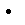
\includegraphics[width=12.05pt,height=12.05pt]{assets/formulas/formula-0034.png}}\penalty0\hspace{0pt}, 最小元记为\hspace{0pt}\penalty0\raisebox{-2pt}{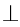
\includegraphics[width=9.65pt,height=13.1pt]{assets/formulas/formula-0035.png}}\penalty0\hspace{0pt}. \hspace{0pt}\penalty0\raisebox{-2pt}{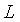
\includegraphics[width=10pt,height=11pt]{assets/formulas/formula-0036.png}}\penalty0\hspace{0pt}上的一个二元关系\hspace{0pt}\penalty0\raisebox{-3pt}{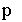
\includegraphics[width=11pt,height=11pt]{assets/formulas/formula-0037.png}}\penalty0\hspace{0pt}定义为, 对\hspace{0pt}\penalty0\raisebox{-4pt}{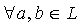
\includegraphics[width=41.55pt,height=13.5pt]{assets/formulas/formula-0038.png}}\penalty0\hspace{0pt},\hspace{0pt}\penalty0\raisebox{-3pt}{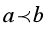
\includegraphics[width=23.7pt,height=14.45pt]{assets/formulas/formula-0039.png}}\penalty0\hspace{0pt}当且仅当对\hspace{0pt}\penalty0\raisebox{-4pt}{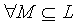
\includegraphics[width=39pt,height=13pt]{assets/formulas/formula-0040.png}}\penalty0\hspace{0pt},\hspace{0pt}\penalty0\raisebox{-3pt}{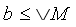
\includegraphics[width=38pt,height=13.05pt]{assets/formulas/formula-0041.png}}\penalty0\hspace{0pt}, 存在一个\hspace{0pt}\penalty0\raisebox{-3pt}{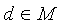
\includegraphics[width=31pt,height=13.05pt]{assets/formulas/formula-0042.png}}\penalty0\hspace{0pt}, 使得\hspace{0pt}\penalty0\raisebox{-3pt}{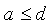
\includegraphics[width=26pt,height=13.05pt]{assets/formulas/formula-0043.png}}\penalty0\hspace{0pt}. 映射\hspace{0pt}\penalty0\raisebox{-5pt}{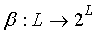
\includegraphics[width=49pt,height=18pt]{assets/formulas/formula-0044.png}}\penalty0\hspace{0pt}定义为\hspace{0pt}\penalty0\raisebox{-6pt}{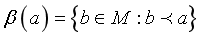
\includegraphics[width=101pt,height=18pt]{assets/formulas/formula-0045.png}}\penalty0\hspace{0pt}, 且满足对\hspace{0pt}\penalty0\raisebox{-6pt}{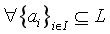
\includegraphics[width=55pt,height=17pt]{assets/formulas/formula-0046.png}}\penalty0\hspace{0pt},\hspace{0pt}\penalty0\raisebox{-12pt}{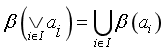
\includegraphics[width=83pt,height=26pt]{assets/formulas/formula-0047.png}}\penalty0\hspace{0pt}\cite{ref7}.

\textbf{定义2.1}\cite{ref8}  \hspace{0pt}\penalty0\raisebox{-2pt}{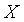
\includegraphics[width=12pt,height=11pt]{assets/formulas/formula-0048.png}}\penalty0\hspace{0pt}上的一个非空子集\hspace{0pt}\penalty0\raisebox{-4pt}{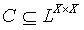
\includegraphics[width=42pt,height=15pt]{assets/formulas/formula-0049.png}}\penalty0\hspace{0pt}称为\hspace{0pt}\penalty0\raisebox{-2pt}{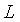
\includegraphics[width=10pt,height=11pt]{assets/formulas/formula-0050.png}}\penalty0\hspace{0pt}-熵,如果它满足以下性质：

（E1）\hspace{0pt}\penalty0\raisebox{-6pt}{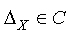
\includegraphics[width=36pt,height=18pt]{assets/formulas/formula-0051.png}}\penalty0\hspace{0pt}；

（E2）如果\hspace{0pt}\penalty0\raisebox{-3pt}{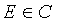
\includegraphics[width=29pt,height=12.05pt]{assets/formulas/formula-0052.png}}\penalty0\hspace{0pt},且\hspace{0pt}\penalty0\raisebox{-2pt}{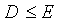
\includegraphics[width=30pt,height=11pt]{assets/formulas/formula-0053.png}}\penalty0\hspace{0pt},则\hspace{0pt}\penalty0\raisebox{-3pt}{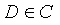
\includegraphics[width=30pt,height=12.05pt]{assets/formulas/formula-0054.png}}\penalty0\hspace{0pt}；

（E3）\hspace{0pt}\penalty0\raisebox{-4pt}{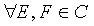
\includegraphics[width=47pt,height=13pt]{assets/formulas/formula-0055.png}}\penalty0\hspace{0pt},则\hspace{0pt}\penalty0\raisebox{-3pt}{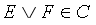
\includegraphics[width=48pt,height=12.05pt]{assets/formulas/formula-0056.png}}\penalty0\hspace{0pt}；

一个\hspace{0pt}\penalty0\raisebox{-2pt}{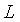
\includegraphics[width=10pt,height=11pt]{assets/formulas/formula-0057.png}}\penalty0\hspace{0pt}-熵\hspace{0pt}\penalty0\raisebox{-4pt}{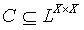
\includegraphics[width=42pt,height=15pt]{assets/formulas/formula-0058.png}}\penalty0\hspace{0pt}称为\hspace{0pt}\penalty0\raisebox{-2pt}{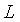
\includegraphics[width=10pt,height=11pt]{assets/formulas/formula-0059.png}}\penalty0\hspace{0pt}-拟粗结构,如果它又满足（E4）：

（E4）\hspace{0pt}\penalty0\raisebox{-4pt}{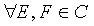
\includegraphics[width=47pt,height=13pt]{assets/formulas/formula-0060.png}}\penalty0\hspace{0pt},则\hspace{0pt}\penalty0\raisebox{-3pt}{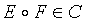
\includegraphics[width=44.05pt,height=12.05pt]{assets/formulas/formula-0061.png}}\penalty0\hspace{0pt}；

一个\hspace{0pt}\penalty0\raisebox{-2pt}{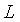
\includegraphics[width=10pt,height=11pt]{assets/formulas/formula-0062.png}}\penalty0\hspace{0pt}-熵\hspace{0pt}\penalty0\raisebox{-4pt}{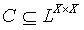
\includegraphics[width=42pt,height=15pt]{assets/formulas/formula-0063.png}}\penalty0\hspace{0pt}称为\hspace{0pt}\penalty0\raisebox{-2pt}{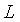
\includegraphics[width=10pt,height=11pt]{assets/formulas/formula-0064.png}}\penalty0\hspace{0pt}-半粗结构,如果它又满足（E5）：

（E5）\hspace{0pt}\penalty0\raisebox{-3pt}{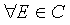
\includegraphics[width=35pt,height=12.05pt]{assets/formulas/formula-0065.png}}\penalty0\hspace{0pt},则\hspace{0pt}\penalty0\raisebox{-3pt}{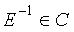
\includegraphics[width=37pt,height=16pt]{assets/formulas/formula-0066.png}}\penalty0\hspace{0pt}.

此外, 一个\hspace{0pt}\penalty0\raisebox{-2pt}{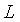
\includegraphics[width=10pt,height=11pt]{assets/formulas/formula-0067.png}}\penalty0\hspace{0pt}-熵\hspace{0pt}\penalty0\raisebox{-4pt}{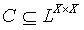
\includegraphics[width=42pt,height=15pt]{assets/formulas/formula-0068.png}}\penalty0\hspace{0pt}称为\hspace{0pt}\penalty0\raisebox{-2pt}{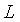
\includegraphics[width=10pt,height=11pt]{assets/formulas/formula-0069.png}}\penalty0\hspace{0pt}-粗结构, 如果它既是\hspace{0pt}\penalty0\raisebox{-2pt}{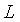
\includegraphics[width=10pt,height=11pt]{assets/formulas/formula-0070.png}}\penalty0\hspace{0pt}-拟粗结构, 又是\hspace{0pt}\penalty0\raisebox{-2pt}{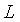
\includegraphics[width=10pt,height=11pt]{assets/formulas/formula-0071.png}}\penalty0\hspace{0pt}-半粗结构.相应地, \hspace{0pt}\penalty0\raisebox{-6pt}{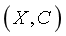
\includegraphics[width=33pt,height=18pt]{assets/formulas/formula-0072.png}}\penalty0\hspace{0pt}又分别称为\hspace{0pt}\penalty0\raisebox{-2pt}{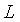
\includegraphics[width=10pt,height=11pt]{assets/formulas/formula-0073.png}}\penalty0\hspace{0pt}-熵空间, \hspace{0pt}\penalty0\raisebox{-2pt}{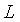
\includegraphics[width=10pt,height=11pt]{assets/formulas/formula-0074.png}}\penalty0\hspace{0pt}-拟粗空间, \hspace{0pt}\penalty0\raisebox{-2pt}{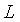
\includegraphics[width=10pt,height=11pt]{assets/formulas/formula-0075.png}}\penalty0\hspace{0pt}-半粗空间, \hspace{0pt}\penalty0\raisebox{-2pt}{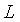
\includegraphics[width=10pt,height=11pt]{assets/formulas/formula-0076.png}}\penalty0\hspace{0pt}-粗空间\cite{ref7}.

\textbf{定义2.2}\cite{ref8}对集合\hspace{0pt}\penalty0\raisebox{-2pt}{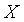
\includegraphics[width=12pt,height=11pt]{assets/formulas/formula-0077.png}}\penalty0\hspace{0pt}及\hspace{0pt}\penalty0\raisebox{-5pt}{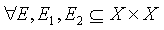
\includegraphics[width=82pt,height=15pt]{assets/formulas/formula-0078.png}}\penalty0\hspace{0pt}, 我们定义

\begin{center}
\noindent \hspace{0pt}\penalty0\raisebox{-7pt}{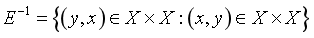
\includegraphics[width=157pt,height=19pt]{assets/formulas/formula-0079.png}}\penalty0\hspace{0pt},
\end{center}
\begin{center}
\noindent \hspace{0pt}\penalty0\raisebox{-7pt}{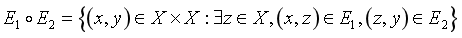
\includegraphics[width=231pt,height=19pt]{assets/formulas/formula-0080.png}}\penalty0\hspace{0pt}.
\end{center}
对于上述运算，其单位元是\hspace{0pt}\penalty0\raisebox{-5pt}{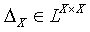
\includegraphics[width=45pt,height=16pt]{assets/formulas/formula-0081.png}}\penalty0\hspace{0pt}，定义为

\begin{center}
\noindent \hspace{0pt}\penalty0\raisebox{-13pt}{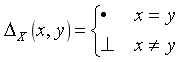
\includegraphics[width=90pt,height=31pt]{assets/formulas/formula-0082.png}}\penalty0\hspace{0pt}. \cite{ref7}
\end{center}
\textbf{定义2.3}\cite{ref9}\textbf{  }映射\hspace{0pt}\penalty0\raisebox{-3pt}{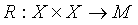
\includegraphics[width=69pt,height=12.05pt]{assets/formulas/formula-0083.png}}\penalty0\hspace{0pt}是\hspace{0pt}\penalty0\raisebox{-2pt}{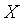
\includegraphics[width=12.05pt,height=11pt]{assets/formulas/formula-0084.png}}\penalty0\hspace{0pt}上一个\hspace{0pt}\penalty0\raisebox{-6pt}{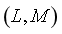
\includegraphics[width=31pt,height=17pt]{assets/formulas/formula-0085.png}}\penalty0\hspace{0pt}-模糊关系, 称为：

（1）自反: \hspace{0pt}\penalty0\raisebox{-6pt}{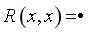
\includegraphics[width=48pt,height=17pt]{assets/formulas/formula-0086.png}}\penalty0\hspace{0pt}；

（2）对称: \hspace{0pt}\penalty0\raisebox{-6pt}{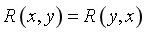
\includegraphics[width=73pt,height=17pt]{assets/formulas/formula-0087.png}}\penalty0\hspace{0pt}；

（3）传递: \hspace{0pt}\penalty0\raisebox{-2pt}{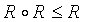
\includegraphics[width=42.95pt,height=11pt]{assets/formulas/formula-0088.png}}\penalty0\hspace{0pt}, 其中\hspace{0pt}\penalty0\raisebox{-11pt}{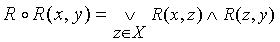
\includegraphics[width=139.95pt,height=21pt]{assets/formulas/formula-0089.png}}\penalty0\hspace{0pt}.

一个满足自反、对称和传递的\hspace{0pt}\penalty0\raisebox{-6pt}{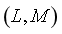
\includegraphics[width=31pt,height=17pt]{assets/formulas/formula-0090.png}}\penalty0\hspace{0pt}-模糊关系\hspace{0pt}\penalty0\raisebox{-2pt}{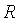
\includegraphics[width=11pt,height=11pt]{assets/formulas/formula-0091.png}}\penalty0\hspace{0pt}称为\hspace{0pt}\penalty0\raisebox{-6pt}{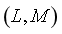
\includegraphics[width=31pt,height=17pt]{assets/formulas/formula-0092.png}}\penalty0\hspace{0pt}-模糊等价关系, 如果\hspace{0pt}\penalty0\raisebox{-3pt}{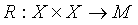
\includegraphics[width=69pt,height=12.05pt]{assets/formulas/formula-0093.png}}\penalty0\hspace{0pt}是\hspace{0pt}\penalty0\raisebox{-2pt}{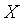
\includegraphics[width=12.05pt,height=11pt]{assets/formulas/formula-0094.png}}\penalty0\hspace{0pt}上一个\hspace{0pt}\penalty0\raisebox{-6pt}{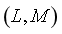
\includegraphics[width=31pt,height=17pt]{assets/formulas/formula-0095.png}}\penalty0\hspace{0pt}-模糊关系, 则称\hspace{0pt}\penalty0\raisebox{-6pt}{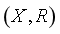
\includegraphics[width=30pt,height=17pt]{assets/formulas/formula-0096.png}}\penalty0\hspace{0pt}为\hspace{0pt}\penalty0\raisebox{-6pt}{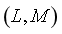
\includegraphics[width=31pt,height=17pt]{assets/formulas/formula-0097.png}}\penalty0\hspace{0pt}-模糊关系空间\cite{ref9}.


\chapter{$(L,M)$-模糊粗结构}
\vspace{0.2cm}
\textbf{定义3.1}  集合\hspace{0pt}\penalty0\raisebox{-2pt}{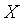
\includegraphics[width=12.05pt,height=11pt]{assets/formulas/formula-0099.png}}\penalty0\hspace{0pt}上的一个\hspace{0pt}\penalty0\raisebox{-4pt}{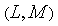
\includegraphics[width=29pt,height=13pt]{assets/formulas/formula-0100.png}}\penalty0\hspace{0pt}-模糊熵结构是一个映射\hspace{0pt}\penalty0\raisebox{-3pt}{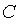
\includegraphics[width=11pt,height=12.05pt]{assets/formulas/formula-0101.png}}\penalty0\hspace{0pt}\hspace{0pt}\penalty0\raisebox{-3pt}{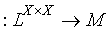
\includegraphics[width=55pt,height=16pt]{assets/formulas/formula-0102.png}}\penalty0\hspace{0pt}满足以下条件：

（ME1）\hspace{0pt}\penalty0\raisebox{-6pt}{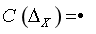
\includegraphics[width=48pt,height=17pt]{assets/formulas/formula-0103.png}}\penalty0\hspace{0pt}；

（ME2）\hspace{0pt}\penalty0\raisebox{-4pt}{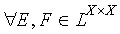
\includegraphics[width=60pt,height=17pt]{assets/formulas/formula-0104.png}}\penalty0\hspace{0pt}, 且\hspace{0pt}\penalty0\raisebox{-2pt}{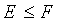
\includegraphics[width=29pt,height=11pt]{assets/formulas/formula-0105.png}}\penalty0\hspace{0pt},则\hspace{0pt}\penalty0\raisebox{-6pt}{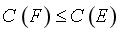
\includegraphics[width=60pt,height=17pt]{assets/formulas/formula-0106.png}}\penalty0\hspace{0pt}；

（ME3）\hspace{0pt}\penalty0\raisebox{-4pt}{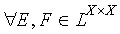
\includegraphics[width=60pt,height=17pt]{assets/formulas/formula-0107.png}}\penalty0\hspace{0pt}, 则\hspace{0pt}\penalty0\raisebox{-6pt}{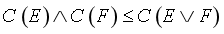
\includegraphics[width=112pt,height=17pt]{assets/formulas/formula-0108.png}}\penalty0\hspace{0pt}；

\quad 一个\hspace{0pt}\penalty0\raisebox{-4pt}{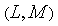
\includegraphics[width=29pt,height=13pt]{assets/formulas/formula-0109.png}}\penalty0\hspace{0pt}-模糊熵结构\hspace{0pt}\penalty0\raisebox{-3pt}{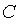
\includegraphics[width=11pt,height=12.05pt]{assets/formulas/formula-0110.png}}\penalty0\hspace{0pt}称为\hspace{0pt}\penalty0\raisebox{-4pt}{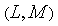
\includegraphics[width=29pt,height=13pt]{assets/formulas/formula-0111.png}}\penalty0\hspace{0pt}-模糊拟粗结构, 若它又满足（ME4）：

（ME4）\hspace{0pt}\penalty0\raisebox{-4pt}{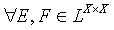
\includegraphics[width=57pt,height=15pt]{assets/formulas/formula-0112.png}}\penalty0\hspace{0pt}, 则\hspace{0pt}\penalty0\raisebox{-6pt}{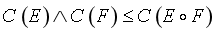
\includegraphics[width=108pt,height=17pt]{assets/formulas/formula-0113.png}}\penalty0\hspace{0pt}；

\quad 一个\hspace{0pt}\penalty0\raisebox{-4pt}{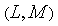
\includegraphics[width=29pt,height=13pt]{assets/formulas/formula-0114.png}}\penalty0\hspace{0pt}-模糊熵结构\hspace{0pt}\penalty0\raisebox{-3pt}{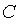
\includegraphics[width=11pt,height=12.05pt]{assets/formulas/formula-0115.png}}\penalty0\hspace{0pt}称为\hspace{0pt}\penalty0\raisebox{-4pt}{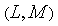
\includegraphics[width=29pt,height=13pt]{assets/formulas/formula-0116.png}}\penalty0\hspace{0pt}-模糊半粗结构, 若它又满足（ME5）：

（ME5）\hspace{0pt}\penalty0\raisebox{-2pt}{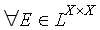
\includegraphics[width=49.95pt,height=15pt]{assets/formulas/formula-0117.png}}\penalty0\hspace{0pt}, 则\hspace{0pt}\penalty0\raisebox{-7pt}{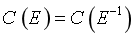
\includegraphics[width=67.95pt,height=19pt]{assets/formulas/formula-0118.png}}\penalty0\hspace{0pt}.

若一个\hspace{0pt}\penalty0\raisebox{-6pt}{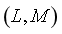
\includegraphics[width=31pt,height=17pt]{assets/formulas/formula-0119.png}}\penalty0\hspace{0pt}-模糊熵结构\hspace{0pt}\penalty0\raisebox{-3pt}{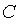
\includegraphics[width=11pt,height=12.05pt]{assets/formulas/formula-0120.png}}\penalty0\hspace{0pt}既是\hspace{0pt}\penalty0\raisebox{-6pt}{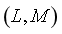
\includegraphics[width=31pt,height=17pt]{assets/formulas/formula-0121.png}}\penalty0\hspace{0pt}-模糊半粗结构, 又是\hspace{0pt}\penalty0\raisebox{-6pt}{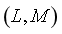
\includegraphics[width=31pt,height=17pt]{assets/formulas/formula-0122.png}}\penalty0\hspace{0pt}-模糊拟粗结构, 则称为\hspace{0pt}\penalty0\raisebox{-6pt}{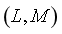
\includegraphics[width=31pt,height=17pt]{assets/formulas/formula-0123.png}}\penalty0\hspace{0pt}-模糊粗结构. 相应地, \hspace{0pt}\penalty0\raisebox{-6pt}{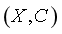
\includegraphics[width=31pt,height=17pt]{assets/formulas/formula-0124.png}}\penalty0\hspace{0pt}分别称为\hspace{0pt}\penalty0\raisebox{-6pt}{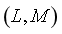
\includegraphics[width=31pt,height=17pt]{assets/formulas/formula-0125.png}}\penalty0\hspace{0pt}-模糊熵空间, \hspace{0pt}\penalty0\raisebox{-6pt}{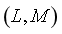
\includegraphics[width=31pt,height=17pt]{assets/formulas/formula-0126.png}}\penalty0\hspace{0pt}-模糊半粗空间, \hspace{0pt}\penalty0\raisebox{-6pt}{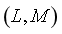
\includegraphics[width=31pt,height=17pt]{assets/formulas/formula-0127.png}}\penalty0\hspace{0pt}-模糊拟粗空间, \hspace{0pt}\penalty0\raisebox{-6pt}{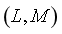
\includegraphics[width=31pt,height=17pt]{assets/formulas/formula-0128.png}}\penalty0\hspace{0pt}-模糊粗空间.

\textbf{注 3.2}  上述定义中的（ME2）和（ME3）可等价于（ME2\&3）：\hspace{0pt}\penalty0\raisebox{-6pt}{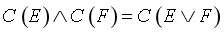
\includegraphics[width=112pt,height=17pt]{assets/formulas/formula-0129.png}}\penalty0\hspace{0pt}.

\textbf{定义3.3}  集合\hspace{0pt}\penalty0\raisebox{-2pt}{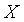
\includegraphics[width=12pt,height=11pt]{assets/formulas/formula-0130.png}}\penalty0\hspace{0pt}上的映射\hspace{0pt}\penalty0\raisebox{-3pt}{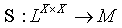
\includegraphics[width=60.95pt,height=13.95pt]{assets/formulas/formula-0131.png}}\penalty0\hspace{0pt}称为一个\hspace{0pt}\penalty0\raisebox{-6pt}{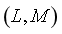
\includegraphics[width=31pt,height=17pt]{assets/formulas/formula-0132.png}}\penalty0\hspace{0pt}-模糊熵结构（或\hspace{0pt}\penalty0\raisebox{-6pt}{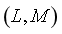
\includegraphics[width=31pt,height=17pt]{assets/formulas/formula-0133.png}}\penalty0\hspace{0pt}-模糊拟粗结构、\hspace{0pt}\penalty0\raisebox{-6pt}{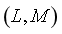
\includegraphics[width=31pt,height=17pt]{assets/formulas/formula-0134.png}}\penalty0\hspace{0pt}-模糊半粗结构、\hspace{0pt}\penalty0\raisebox{-6pt}{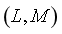
\includegraphics[width=31pt,height=17pt]{assets/formulas/formula-0135.png}}\penalty0\hspace{0pt}-模糊粗结构）\hspace{0pt}\penalty0\raisebox{-3pt}{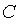
\includegraphics[width=11pt,height=12.05pt]{assets/formulas/formula-0136.png}}\penalty0\hspace{0pt}的基, 若它满足：对\hspace{0pt}\penalty0\raisebox{-2pt}{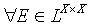
\includegraphics[width=46pt,height=13pt]{assets/formulas/formula-0137.png}}\penalty0\hspace{0pt}, \hspace{0pt}\penalty0\raisebox{-7pt}{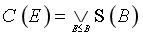
\includegraphics[width=71.05pt,height=18pt]{assets/formulas/formula-0138.png}}\penalty0\hspace{0pt}.

\textbf{定义3.4}  集合\hspace{0pt}\penalty0\raisebox{-2pt}{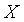
\includegraphics[width=12pt,height=11pt]{assets/formulas/formula-0139.png}}\penalty0\hspace{0pt}上的映射\hspace{0pt}\penalty0\raisebox{-3pt}{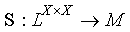
\includegraphics[width=65pt,height=16pt]{assets/formulas/formula-0140.png}}\penalty0\hspace{0pt}称为一个\hspace{0pt}\penalty0\raisebox{-6pt}{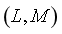
\includegraphics[width=31pt,height=17pt]{assets/formulas/formula-0141.png}}\penalty0\hspace{0pt}-模糊熵结构的基, 若它满足：

\quad （B1）\hspace{0pt}\penalty0\raisebox{-8pt}{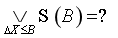
\includegraphics[width=59pt,height=19pt]{assets/formulas/formula-0142.png}}\penalty0\hspace{0pt}；

\quad （B2）\hspace{0pt}\penalty0\raisebox{-5pt}{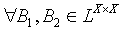
\includegraphics[width=62pt,height=16pt]{assets/formulas/formula-0143.png}}\penalty0\hspace{0pt},\hspace{0pt}\penalty0\raisebox{-10pt}{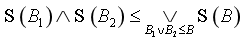
\includegraphics[width=121.95pt,height=21pt]{assets/formulas/formula-0144.png}}\penalty0\hspace{0pt}；

\quad \hspace{0pt}\penalty0\raisebox{-3pt}{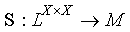
\includegraphics[width=65pt,height=16pt]{assets/formulas/formula-0145.png}}\penalty0\hspace{0pt}称为一个\hspace{0pt}\penalty0\raisebox{-6pt}{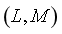
\includegraphics[width=31pt,height=17pt]{assets/formulas/formula-0146.png}}\penalty0\hspace{0pt}-模糊拟粗结构的基, 如果它还满足（B3）：

\quad （B3）\hspace{0pt}\penalty0\raisebox{-5pt}{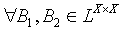
\includegraphics[width=62pt,height=16pt]{assets/formulas/formula-0147.png}}\penalty0\hspace{0pt}, \hspace{0pt}\penalty0\raisebox{-10pt}{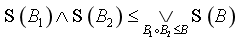
\includegraphics[width=120pt,height=21pt]{assets/formulas/formula-0148.png}}\penalty0\hspace{0pt}；

\quad \hspace{0pt}\penalty0\raisebox{-3pt}{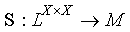
\includegraphics[width=65pt,height=16pt]{assets/formulas/formula-0149.png}}\penalty0\hspace{0pt}称为一个\hspace{0pt}\penalty0\raisebox{-6pt}{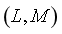
\includegraphics[width=31pt,height=17pt]{assets/formulas/formula-0150.png}}\penalty0\hspace{0pt}-模糊半粗结构的基, 如果它还满足（B4）：

\quad （B4）\hspace{0pt}\penalty0\raisebox{-2pt}{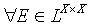
\includegraphics[width=46pt,height=13pt]{assets/formulas/formula-0151.png}}\penalty0\hspace{0pt}, \hspace{0pt}\penalty0\raisebox{-9pt}{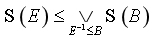
\includegraphics[width=77pt,height=20pt]{assets/formulas/formula-0152.png}}\penalty0\hspace{0pt}；

若\hspace{0pt}\penalty0\raisebox{-2pt}{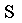
\includegraphics[width=11pt,height=11.05pt]{assets/formulas/formula-0153.png}}\penalty0\hspace{0pt}同时满足（B1）（B4）, 则称为\hspace{0pt}\penalty0\raisebox{-6pt}{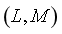
\includegraphics[width=31pt,height=17pt]{assets/formulas/formula-0154.png}}\penalty0\hspace{0pt}-模糊粗结构的基.

由一个\hspace{0pt}\penalty0\raisebox{-6pt}{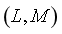
\includegraphics[width=31pt,height=17pt]{assets/formulas/formula-0155.png}}\penalty0\hspace{0pt}-模糊熵结构（或\hspace{0pt}\penalty0\raisebox{-6pt}{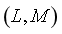
\includegraphics[width=31pt,height=17pt]{assets/formulas/formula-0156.png}}\penalty0\hspace{0pt}-模糊拟粗结构、\hspace{0pt}\penalty0\raisebox{-6pt}{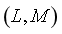
\includegraphics[width=31pt,height=17pt]{assets/formulas/formula-0157.png}}\penalty0\hspace{0pt}-模糊半粗结构、\hspace{0pt}\penalty0\raisebox{-6pt}{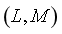
\includegraphics[width=31pt,height=17pt]{assets/formulas/formula-0158.png}}\penalty0\hspace{0pt}-模糊粗结构）\hspace{0pt}\penalty0\raisebox{-3pt}{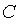
\includegraphics[width=11pt,height=12.05pt]{assets/formulas/formula-0159.png}}\penalty0\hspace{0pt}的基\hspace{0pt}\penalty0\raisebox{-3pt}{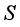
\includegraphics[width=10pt,height=13.05pt]{assets/formulas/formula-0160.png}}\penalty0\hspace{0pt}, 可以通过\hspace{0pt}\penalty0\raisebox{-8pt}{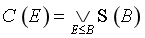
\includegraphics[width=72.05pt,height=19pt]{assets/formulas/formula-0161.png}}\penalty0\hspace{0pt}生成一个\hspace{0pt}\penalty0\raisebox{-6pt}{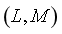
\includegraphics[width=31pt,height=17pt]{assets/formulas/formula-0162.png}}\penalty0\hspace{0pt}-模糊熵结构（或\hspace{0pt}\penalty0\raisebox{-6pt}{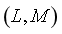
\includegraphics[width=31pt,height=17pt]{assets/formulas/formula-0163.png}}\penalty0\hspace{0pt}-模糊拟粗结构, \hspace{0pt}\penalty0\raisebox{-6pt}{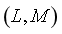
\includegraphics[width=31pt,height=17pt]{assets/formulas/formula-0164.png}}\penalty0\hspace{0pt}-模糊半粗结构,\hspace{0pt}\penalty0\raisebox{-6pt}{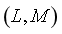
\includegraphics[width=31pt,height=17pt]{assets/formulas/formula-0165.png}}\penalty0\hspace{0pt}-模糊粗结构）.

\textbf{定义3.5}  两个\hspace{0pt}\penalty0\raisebox{-6pt}{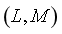
\includegraphics[width=31pt,height=17pt]{assets/formulas/formula-0166.png}}\penalty0\hspace{0pt}-模糊熵空间之间的映射\hspace{0pt}\penalty0\raisebox{-6pt}{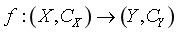
\includegraphics[width=89pt,height=17pt]{assets/formulas/formula-0167.png}}\penalty0\hspace{0pt}称为：

\quad （1）\hspace{0pt}\penalty0\raisebox{-6pt}{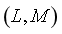
\includegraphics[width=31pt,height=17pt]{assets/formulas/formula-0168.png}}\penalty0\hspace{0pt}-模糊保有界映射, 若对\hspace{0pt}\penalty0\raisebox{-2pt}{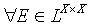
\includegraphics[width=46pt,height=13pt]{assets/formulas/formula-0169.png}}\penalty0\hspace{0pt}, 有\hspace{0pt}\penalty0\raisebox{-7pt}{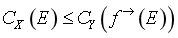
\includegraphics[width=89pt,height=19pt]{assets/formulas/formula-0170.png}}\penalty0\hspace{0pt}；

\quad （2）\hspace{0pt}\penalty0\raisebox{-6pt}{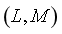
\includegraphics[width=31pt,height=17pt]{assets/formulas/formula-0171.png}}\penalty0\hspace{0pt}-模糊有效逆紧映射, 若对\hspace{0pt}\penalty0\raisebox{-2pt}{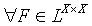
\includegraphics[width=46pt,height=13pt]{assets/formulas/formula-0172.png}}\penalty0\hspace{0pt},有\hspace{0pt}\penalty0\raisebox{-7pt}{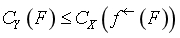
\includegraphics[width=90pt,height=19pt]{assets/formulas/formula-0173.png}}\penalty0\hspace{0pt}；

\quad （3）\hspace{0pt}\penalty0\raisebox{-6pt}{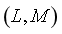
\includegraphics[width=31pt,height=17pt]{assets/formulas/formula-0174.png}}\penalty0\hspace{0pt}-模糊粗蕴含映射, 若\hspace{0pt}\penalty0\raisebox{-5pt}{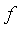
\includegraphics[width=11pt,height=15pt]{assets/formulas/formula-0175.png}}\penalty0\hspace{0pt}既是\hspace{0pt}\penalty0\raisebox{-6pt}{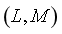
\includegraphics[width=31pt,height=17pt]{assets/formulas/formula-0176.png}}\penalty0\hspace{0pt}-模糊保有界, 又是\hspace{0pt}\penalty0\raisebox{-6pt}{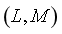
\includegraphics[width=31pt,height=17pt]{assets/formulas/formula-0177.png}}\penalty0\hspace{0pt}-模糊有效逆紧的；

\quad （4）\hspace{0pt}\penalty0\raisebox{-6pt}{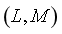
\includegraphics[width=31pt,height=17pt]{assets/formulas/formula-0178.png}}\penalty0\hspace{0pt}-模糊粗映射, 若\hspace{0pt}\penalty0\raisebox{-5pt}{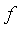
\includegraphics[width=11pt,height=15pt]{assets/formulas/formula-0179.png}}\penalty0\hspace{0pt}既是\hspace{0pt}\penalty0\raisebox{-6pt}{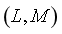
\includegraphics[width=31pt,height=17pt]{assets/formulas/formula-0180.png}}\penalty0\hspace{0pt}-模糊保有界的, 又是\hspace{0pt}\penalty0\raisebox{-6pt}{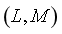
\includegraphics[width=31pt,height=17pt]{assets/formulas/formula-0181.png}}\penalty0\hspace{0pt}-模糊有效逆紧的.

\textbf{命题3.6}  已知\hspace{0pt}\penalty0\raisebox{-6pt}{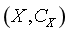
\includegraphics[width=35pt,height=17pt]{assets/formulas/formula-0182.png}}\penalty0\hspace{0pt}和\hspace{0pt}\penalty0\raisebox{-6pt}{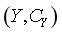
\includegraphics[width=31pt,height=17pt]{assets/formulas/formula-0183.png}}\penalty0\hspace{0pt}是两个\hspace{0pt}\penalty0\raisebox{-6pt}{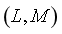
\includegraphics[width=31pt,height=17pt]{assets/formulas/formula-0184.png}}\penalty0\hspace{0pt}-模糊熵空间, 映射\hspace{0pt}\penalty0\raisebox{-5pt}{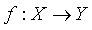
\includegraphics[width=46pt,height=15pt]{assets/formulas/formula-0185.png}}\penalty0\hspace{0pt},\hspace{0pt}\penalty0\raisebox{-6pt}{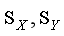
\includegraphics[width=31.95pt,height=18pt]{assets/formulas/formula-0186.png}}\penalty0\hspace{0pt}分别是\hspace{0pt}\penalty0\raisebox{-6pt}{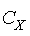
\includegraphics[width=15pt,height=18pt]{assets/formulas/formula-0187.png}}\penalty0\hspace{0pt}和\hspace{0pt}\penalty0\raisebox{-6pt}{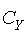
\includegraphics[width=13.95pt,height=18pt]{assets/formulas/formula-0188.png}}\penalty0\hspace{0pt}的基, 则：

\quad （1）\hspace{0pt}\penalty0\raisebox{-5pt}{\includegraphics[width=11pt,height=15pt]{assets/formulas/formula-0189.png}}\penalty0\hspace{0pt}是\hspace{0pt}\penalty0\raisebox{-6pt}{\includegraphics[width=31pt,height=17pt]{assets/formulas/formula-0190.png}}\penalty0\hspace{0pt}-模糊保有界映射当且仅当\hspace{0pt}\penalty0\raisebox{-7pt}{\includegraphics[width=89pt,height=19pt]{assets/formulas/formula-0191.png}}\penalty0\hspace{0pt}；

\quad （2）\hspace{0pt}\penalty0\raisebox{-5pt}{\includegraphics[width=11pt,height=15pt]{assets/formulas/formula-0192.png}}\penalty0\hspace{0pt}是\hspace{0pt}\penalty0\raisebox{-6pt}{\includegraphics[width=31pt,height=17pt]{assets/formulas/formula-0193.png}}\penalty0\hspace{0pt}-模糊有效逆紧映射当且仅当\hspace{0pt}\penalty0\raisebox{-7pt}{\includegraphics[width=91pt,height=19pt]{assets/formulas/formula-0194.png}}\penalty0\hspace{0pt}.

证明 （1）“必要性”: 由于\hspace{0pt}\penalty0\raisebox{-8pt}{\includegraphics[width=82pt,height=19pt]{assets/formulas/formula-0195.png}}\penalty0\hspace{0pt}, 故\hspace{0pt}\penalty0\raisebox{-7pt}{\includegraphics[width=126pt,height=19pt]{assets/formulas/formula-0196.png}}\penalty0\hspace{0pt}.

“充分性”: \hspace{0pt}\penalty0\raisebox{-8pt}{\includegraphics[width=211pt,height=20pt]{assets/formulas/formula-0197.png}}\penalty0\hspace{0pt}, 故得证\hspace{0pt}\penalty0\raisebox{-5pt}{\includegraphics[width=11pt,height=15pt]{assets/formulas/formula-0198.png}}\penalty0\hspace{0pt}是\hspace{0pt}\penalty0\raisebox{-6pt}{\includegraphics[width=31pt,height=17pt]{assets/formulas/formula-0199.png}}\penalty0\hspace{0pt}-模糊保有界映射.

（2）“必要性”: 由于\hspace{0pt}\penalty0\raisebox{-8pt}{\includegraphics[width=81pt,height=19pt]{assets/formulas/formula-0200.png}}\penalty0\hspace{0pt}, 则\hspace{0pt}\penalty0\raisebox{-7pt}{\includegraphics[width=128pt,height=19pt]{assets/formulas/formula-0201.png}}\penalty0\hspace{0pt}.

“充分性”: 因\hspace{0pt}\penalty0\raisebox{-8pt}{\includegraphics[width=216pt,height=20pt]{assets/formulas/formula-0202.png}}\penalty0\hspace{0pt}, 故\hspace{0pt}\penalty0\raisebox{-5pt}{\includegraphics[width=11pt,height=15pt]{assets/formulas/formula-0203.png}}\penalty0\hspace{0pt}是\hspace{0pt}\penalty0\raisebox{-6pt}{\includegraphics[width=31pt,height=17pt]{assets/formulas/formula-0204.png}}\penalty0\hspace{0pt}-模糊有效逆紧映射.

\textbf{定义3.7}  \hspace{0pt}\penalty0\raisebox{-6pt}{\includegraphics[width=35pt,height=17pt]{assets/formulas/formula-0205.png}}\penalty0\hspace{0pt}和\hspace{0pt}\penalty0\raisebox{-6pt}{\includegraphics[width=31pt,height=17pt]{assets/formulas/formula-0206.png}}\penalty0\hspace{0pt}是两个\hspace{0pt}\penalty0\raisebox{-6pt}{\includegraphics[width=31pt,height=17pt]{assets/formulas/formula-0207.png}}\penalty0\hspace{0pt}-模糊粗空间,

（1）\hspace{0pt}\penalty0\raisebox{-6pt}{\includegraphics[width=77pt,height=17pt]{assets/formulas/formula-0208.png}}\penalty0\hspace{0pt}是两个映射, \hspace{0pt}\penalty0\raisebox{-5pt}{\includegraphics[width=11pt,height=15pt]{assets/formulas/formula-0209.png}}\penalty0\hspace{0pt}和\hspace{0pt}\penalty0\raisebox{-5pt}{\includegraphics[width=10pt,height=12pt]{assets/formulas/formula-0210.png}}\penalty0\hspace{0pt}称为有界接近的, 表示为\hspace{0pt}\penalty0\raisebox{-5pt}{\includegraphics[width=28.05pt,height=15pt]{assets/formulas/formula-0211.png}}\penalty0\hspace{0pt}, 如果

\begin{center}
\noindent \hspace{0pt}\penalty0\raisebox{-11pt}{\includegraphics[width=175.95pt,height=26pt]{assets/formulas/formula-0212.png}}\penalty0\hspace{0pt}；
\end{center}
（2）映射\hspace{0pt}\penalty0\raisebox{-6pt}{\includegraphics[width=89pt,height=17pt]{assets/formulas/formula-0213.png}}\penalty0\hspace{0pt}称为\hspace{0pt}\penalty0\raisebox{-6pt}{\includegraphics[width=31pt,height=17pt]{assets/formulas/formula-0214.png}}\penalty0\hspace{0pt}-模糊粗等价, 若对\hspace{0pt}\penalty0\raisebox{-5pt}{\includegraphics[width=51pt,height=16pt]{assets/formulas/formula-0215.png}}\penalty0\hspace{0pt}, \newline 有\hspace{0pt}\penalty0\raisebox{-7pt}{\includegraphics[width=100pt,height=19pt]{assets/formulas/formula-0216.png}}\penalty0\hspace{0pt}, 且存在映射\hspace{0pt}\penalty0\raisebox{-6pt}{\includegraphics[width=89pt,height=17pt]{assets/formulas/formula-0217.png}}\penalty0\hspace{0pt}, \newline 满足对\hspace{0pt}\penalty0\raisebox{-5pt}{\includegraphics[width=47pt,height=16pt]{assets/formulas/formula-0218.png}}\penalty0\hspace{0pt},\hspace{0pt}\penalty0\raisebox{-7pt}{\includegraphics[width=96.95pt,height=19pt]{assets/formulas/formula-0219.png}}\penalty0\hspace{0pt}, 有\hspace{0pt}\penalty0\raisebox{-6pt}{\includegraphics[width=49pt,height=18pt]{assets/formulas/formula-0220.png}}\penalty0\hspace{0pt}, \hspace{0pt}\penalty0\raisebox{-6pt}{\includegraphics[width=49.95pt,height=18pt]{assets/formulas/formula-0221.png}}\penalty0\hspace{0pt}. （即\hspace{0pt}\penalty0\raisebox{-5pt}{\includegraphics[width=11pt,height=15pt]{assets/formulas/formula-0222.png}}\penalty0\hspace{0pt}是\hspace{0pt}\penalty0\raisebox{-6pt}{\includegraphics[width=31pt,height=17pt]{assets/formulas/formula-0223.png}}\penalty0\hspace{0pt}-模糊保有界映射, 存在\hspace{0pt}\penalty0\raisebox{-5pt}{\includegraphics[width=10pt,height=12pt]{assets/formulas/formula-0224.png}}\penalty0\hspace{0pt}也是\hspace{0pt}\penalty0\raisebox{-6pt}{\includegraphics[width=31pt,height=17pt]{assets/formulas/formula-0225.png}}\penalty0\hspace{0pt}-模糊保有界映射, 使得\hspace{0pt}\penalty0\raisebox{-6pt}{\includegraphics[width=49pt,height=18pt]{assets/formulas/formula-0226.png}}\penalty0\hspace{0pt}, \hspace{0pt}\penalty0\raisebox{-6pt}{\includegraphics[width=49.95pt,height=18pt]{assets/formulas/formula-0227.png}}\penalty0\hspace{0pt}. ）

\textbf{命题3.8  }\hspace{0pt}\penalty0\raisebox{-6pt}{\includegraphics[width=77pt,height=17pt]{assets/formulas/formula-0228.png}}\penalty0\hspace{0pt}是两个映射, 若\hspace{0pt}\penalty0\raisebox{-5pt}{\includegraphics[width=11pt,height=15pt]{assets/formulas/formula-0229.png}}\penalty0\hspace{0pt}和\hspace{0pt}\penalty0\raisebox{-5pt}{\includegraphics[width=10pt,height=12pt]{assets/formulas/formula-0230.png}}\penalty0\hspace{0pt}是有界接近的, 则映射\hspace{0pt}\penalty0\raisebox{-5pt}{\includegraphics[width=11pt,height=15pt]{assets/formulas/formula-0231.png}}\penalty0\hspace{0pt}与\hspace{0pt}\penalty0\raisebox{-5pt}{\includegraphics[width=10pt,height=12pt]{assets/formulas/formula-0232.png}}\penalty0\hspace{0pt}等价.

证明 “自反性”: 由于

\begin{center}
\noindent \hspace{0pt}\penalty0\raisebox{-11pt}{\includegraphics[width=307pt,height=26pt]{assets/formulas/formula-0233.png}}\penalty0\hspace{0pt},
\end{center}
即\hspace{0pt}\penalty0\raisebox{-5pt}{\includegraphics[width=29pt,height=15pt]{assets/formulas/formula-0234.png}}\penalty0\hspace{0pt},满足自反性.

“对称性”: 假设两个映射\hspace{0pt}\penalty0\raisebox{-5pt}{\includegraphics[width=21pt,height=15pt]{assets/formulas/formula-0235.png}}\penalty0\hspace{0pt}满足\hspace{0pt}\penalty0\raisebox{-5pt}{\includegraphics[width=28.05pt,height=15pt]{assets/formulas/formula-0236.png}}\penalty0\hspace{0pt}, 则

\begin{center}
\noindent \hspace{0pt}\penalty0\raisebox{-11pt}{\includegraphics[width=348pt,height=26pt]{assets/formulas/formula-0237.png}}\penalty0\hspace{0pt},
\end{center}
故\hspace{0pt}\penalty0\raisebox{-5pt}{\includegraphics[width=28.05pt,height=15pt]{assets/formulas/formula-0238.png}}\penalty0\hspace{0pt}得证, 满足对称性.

“传递性”: 假设又存在一个映射\hspace{0pt}\penalty0\raisebox{-6pt}{\includegraphics[width=65pt,height=17pt]{assets/formulas/formula-0239.png}}\penalty0\hspace{0pt}满足\hspace{0pt}\penalty0\raisebox{-5pt}{\includegraphics[width=28.05pt,height=15pt]{assets/formulas/formula-0240.png}}\penalty0\hspace{0pt}且\hspace{0pt}\penalty0\raisebox{-5pt}{\includegraphics[width=27pt,height=15pt]{assets/formulas/formula-0241.png}}\penalty0\hspace{0pt}, 则

\begin{center}
\noindent \hspace{0pt}\penalty0\raisebox{-11pt}{\includegraphics[width=173pt,height=26pt]{assets/formulas/formula-0242.png}}\penalty0\hspace{0pt}, \hspace{0pt}\penalty0\raisebox{-11pt}{\includegraphics[width=170pt,height=26pt]{assets/formulas/formula-0243.png}}\penalty0\hspace{0pt},
\end{center}
又设\hspace{0pt}\penalty0\raisebox{-6pt}{\includegraphics[width=49pt,height=17pt]{assets/formulas/formula-0244.png}}\penalty0\hspace{0pt}, 满足

\begin{center}
\noindent \hspace{0pt}\penalty0\raisebox{-11pt}{\includegraphics[width=174pt,height=26pt]{assets/formulas/formula-0245.png}}\penalty0\hspace{0pt}, \hspace{0pt}\penalty0\raisebox{-11pt}{\includegraphics[width=170pt,height=26pt]{assets/formulas/formula-0246.png}}\penalty0\hspace{0pt},
\end{center}
则存在\hspace{0pt}\penalty0\raisebox{-6pt}{\includegraphics[width=42pt,height=19pt]{assets/formulas/formula-0247.png}}\penalty0\hspace{0pt}, 使得\hspace{0pt}\penalty0\raisebox{-9pt}{\includegraphics[width=142pt,height=23pt]{assets/formulas/formula-0248.png}}\penalty0\hspace{0pt}, 且\hspace{0pt}\penalty0\raisebox{-6pt}{\includegraphics[width=47pt,height=17pt]{assets/formulas/formula-0249.png}}\penalty0\hspace{0pt}, 同理, 存在\hspace{0pt}\penalty0\raisebox{-6pt}{\includegraphics[width=42.95pt,height=19pt]{assets/formulas/formula-0250.png}}\penalty0\hspace{0pt}, 使得\hspace{0pt}\penalty0\raisebox{-9pt}{\includegraphics[width=142pt,height=23pt]{assets/formulas/formula-0251.png}}\penalty0\hspace{0pt}, 且\hspace{0pt}\penalty0\raisebox{-6pt}{\includegraphics[width=49pt,height=17pt]{assets/formulas/formula-0252.png}}\penalty0\hspace{0pt}. 令\hspace{0pt}\penalty0\raisebox{-6pt}{\includegraphics[width=49.95pt,height=18pt]{assets/formulas/formula-0253.png}}\penalty0\hspace{0pt}, \newline 显然\hspace{0pt}\penalty0\raisebox{-6pt}{\includegraphics[width=143pt,height=17pt]{assets/formulas/formula-0254.png}}\penalty0\hspace{0pt},

\begin{center}
\noindent \hspace{0pt}\penalty0\raisebox{-8pt}{\includegraphics[width=379pt,height=19pt]{assets/formulas/formula-0255.png}}\penalty0\hspace{0pt},
\end{center}
得\hspace{0pt}\penalty0\raisebox{-9pt}{\includegraphics[width=136pt,height=23pt]{assets/formulas/formula-0256.png}}\penalty0\hspace{0pt}. 故\hspace{0pt}\penalty0\raisebox{-9pt}{\includegraphics[width=136pt,height=23pt]{assets/formulas/formula-0257.png}}\penalty0\hspace{0pt}, 则

\begin{center}
\noindent \hspace{0pt}\penalty0\raisebox{-10pt}{\includegraphics[width=164pt,height=24.95pt]{assets/formulas/formula-0258.png}}\penalty0\hspace{0pt},
\end{center}
满足传递性.

\textbf{例 }\textbf{3}\textbf{-1}\textbf{  }映射\hspace{0pt}\penalty0\raisebox{-3pt}{\includegraphics[width=69pt,height=12.05pt]{assets/formulas/formula-0259.png}}\penalty0\hspace{0pt}是\hspace{0pt}\penalty0\raisebox{-2pt}{\includegraphics[width=12.05pt,height=11pt]{assets/formulas/formula-0260.png}}\penalty0\hspace{0pt}上一个\hspace{0pt}\penalty0\raisebox{-6pt}{\includegraphics[width=31pt,height=17pt]{assets/formulas/formula-0261.png}}\penalty0\hspace{0pt}-模糊关系, 定义

\begin{center}
\noindent \hspace{0pt}\penalty0\raisebox{-2pt}{\includegraphics[width=49pt,height=15pt]{assets/formulas/formula-0262.png}}\penalty0\hspace{0pt}, \hspace{0pt}\penalty0\raisebox{-13pt}{\includegraphics[width=87pt,height=31pt]{assets/formulas/formula-0263.png}}\penalty0\hspace{0pt},
\end{center}
则:

（1）若\hspace{0pt}\penalty0\raisebox{-2pt}{\includegraphics[width=11pt,height=11pt]{assets/formulas/formula-0264.png}}\penalty0\hspace{0pt}为自反的, 则\hspace{0pt}\penalty0\raisebox{-6pt}{\includegraphics[width=13.95pt,height=18pt]{assets/formulas/formula-0265.png}}\penalty0\hspace{0pt}是\hspace{0pt}\penalty0\raisebox{-6pt}{\includegraphics[width=31pt,height=17pt]{assets/formulas/formula-0266.png}}\penalty0\hspace{0pt}-模糊熵结构；

（2）若\hspace{0pt}\penalty0\raisebox{-2pt}{\includegraphics[width=11pt,height=11pt]{assets/formulas/formula-0267.png}}\penalty0\hspace{0pt}为对称的, 则\hspace{0pt}\penalty0\raisebox{-6pt}{\includegraphics[width=13.95pt,height=18pt]{assets/formulas/formula-0268.png}}\penalty0\hspace{0pt}是\hspace{0pt}\penalty0\raisebox{-6pt}{\includegraphics[width=31pt,height=17pt]{assets/formulas/formula-0269.png}}\penalty0\hspace{0pt}-模糊半粗结构；

（3）若\hspace{0pt}\penalty0\raisebox{-2pt}{\includegraphics[width=11pt,height=11pt]{assets/formulas/formula-0270.png}}\penalty0\hspace{0pt}为传递的, 则\hspace{0pt}\penalty0\raisebox{-6pt}{\includegraphics[width=13.95pt,height=18pt]{assets/formulas/formula-0271.png}}\penalty0\hspace{0pt}是\hspace{0pt}\penalty0\raisebox{-6pt}{\includegraphics[width=31pt,height=17pt]{assets/formulas/formula-0272.png}}\penalty0\hspace{0pt}-模糊拟粗结构；

（4）若\hspace{0pt}\penalty0\raisebox{-2pt}{\includegraphics[width=11pt,height=11pt]{assets/formulas/formula-0273.png}}\penalty0\hspace{0pt}是\hspace{0pt}\penalty0\raisebox{-6pt}{\includegraphics[width=31pt,height=17pt]{assets/formulas/formula-0274.png}}\penalty0\hspace{0pt}-模糊等价关系, 则\hspace{0pt}\penalty0\raisebox{-6pt}{\includegraphics[width=13.95pt,height=18pt]{assets/formulas/formula-0275.png}}\penalty0\hspace{0pt}是\hspace{0pt}\penalty0\raisebox{-6pt}{\includegraphics[width=31pt,height=17pt]{assets/formulas/formula-0276.png}}\penalty0\hspace{0pt}-模糊粗结构.


\chapter{$(L,M)$-模糊球结构}
\vspace{0.2cm}
\textbf{定义}\textbf{4}\textbf{.1}  （1）一个映射\hspace{0pt}\penalty0\raisebox{-3pt}{\includegraphics[width=78.95pt,height=12pt]{assets/formulas/formula-0278.png}}\penalty0\hspace{0pt}称为集合\hspace{0pt}\penalty0\raisebox{-2pt}{\includegraphics[width=12pt,height=11pt]{assets/formulas/formula-0279.png}}\penalty0\hspace{0pt}上关于集合\hspace{0pt}\penalty0\raisebox{-2pt}{\includegraphics[width=11pt,height=11pt]{assets/formulas/formula-0280.png}}\penalty0\hspace{0pt}的一个\hspace{0pt}\penalty0\raisebox{-2pt}{\includegraphics[width=10pt,height=11pt]{assets/formulas/formula-0281.png}}\penalty0\hspace{0pt}-球映射,如果满足：\hspace{0pt}\penalty0\raisebox{-3pt}{\includegraphics[width=34pt,height=12pt]{assets/formulas/formula-0282.png}}\penalty0\hspace{0pt}, \hspace{0pt}\penalty0\raisebox{-2pt}{\includegraphics[width=31.95pt,height=11pt]{assets/formulas/formula-0283.png}}\penalty0\hspace{0pt}, 有\hspace{0pt}\penalty0\raisebox{-6pt}{\includegraphics[width=57pt,height=17pt]{assets/formulas/formula-0284.png}}\penalty0\hspace{0pt}. 进一步, 记\hspace{0pt}\penalty0\raisebox{-7pt}{\includegraphics[width=101pt,height=19pt]{assets/formulas/formula-0285.png}}\penalty0\hspace{0pt}是二元映射族,其中二元映射\hspace{0pt}\penalty0\raisebox{-5pt}{\includegraphics[width=66pt,height=15pt]{assets/formulas/formula-0286.png}}\penalty0\hspace{0pt}定义为：\hspace{0pt}\penalty0\raisebox{-5pt}{\includegraphics[width=42.95pt,height=13.95pt]{assets/formulas/formula-0287.png}}\penalty0\hspace{0pt}, 有\hspace{0pt}\penalty0\raisebox{-6pt}{\includegraphics[width=85.95pt,height=17pt]{assets/formulas/formula-0288.png}}\penalty0\hspace{0pt}.

（2）称映射\hspace{0pt}\penalty0\raisebox{-5pt}{\includegraphics[width=59pt,height=15pt]{assets/formulas/formula-0289.png}}\penalty0\hspace{0pt}为\hspace{0pt}\penalty0\raisebox{-3pt}{\includegraphics[width=11pt,height=12pt]{assets/formulas/formula-0290.png}}\penalty0\hspace{0pt}上的\hspace{0pt}\penalty0\raisebox{-5pt}{\includegraphics[width=31pt,height=15pt]{assets/formulas/formula-0291.png}}\penalty0\hspace{0pt}-模糊球结构, 若对\hspace{0pt}\penalty0\raisebox{-4pt}{\includegraphics[width=38pt,height=13pt]{assets/formulas/formula-0292.png}}\penalty0\hspace{0pt}, 有

\begin{center}
\noindent \hspace{0pt}\penalty0\raisebox{-6pt}{\includegraphics[width=138pt,height=17pt]{assets/formulas/formula-0293.png}}\penalty0\hspace{0pt}.
\end{center}
对于\hspace{0pt}\penalty0\raisebox{-2pt}{\includegraphics[width=12pt,height=11pt]{assets/formulas/formula-0294.png}}\penalty0\hspace{0pt}上的关于集合\hspace{0pt}\penalty0\raisebox{-2pt}{\includegraphics[width=11pt,height=11pt]{assets/formulas/formula-0295.png}}\penalty0\hspace{0pt}的一个\hspace{0pt}\penalty0\raisebox{-2pt}{\includegraphics[width=10pt,height=11pt]{assets/formulas/formula-0296.png}}\penalty0\hspace{0pt}-球映射\hspace{0pt}\penalty0\raisebox{-3pt}{\includegraphics[width=77pt,height=12pt]{assets/formulas/formula-0297.png}}\penalty0\hspace{0pt}和一个\hspace{0pt}\penalty0\raisebox{-5pt}{\includegraphics[width=31pt,height=15pt]{assets/formulas/formula-0298.png}}\penalty0\hspace{0pt}-模糊球结构\hspace{0pt}\penalty0\raisebox{-5pt}{\includegraphics[width=59pt,height=15pt]{assets/formulas/formula-0299.png}}\penalty0\hspace{0pt}, 称四元组\hspace{0pt}\penalty0\raisebox{-6pt}{\includegraphics[width=58pt,height=17pt]{assets/formulas/formula-0300.png}}\penalty0\hspace{0pt}为一个\hspace{0pt}\penalty0\raisebox{-5pt}{\includegraphics[width=31pt,height=15pt]{assets/formulas/formula-0301.png}}\penalty0\hspace{0pt}-模糊球系统.

\textbf{定义}\textbf{4}\textbf{.2  }\hspace{0pt}\penalty0\raisebox{-6pt}{\includegraphics[width=77pt,height=17pt]{assets/formulas/formula-0302.png}}\penalty0\hspace{0pt}是一个\hspace{0pt}\penalty0\raisebox{-5pt}{\includegraphics[width=31pt,height=15pt]{assets/formulas/formula-0303.png}}\penalty0\hspace{0pt}-模糊球系统, 称\hspace{0pt}\penalty0\raisebox{-3pt}{\includegraphics[width=11pt,height=12pt]{assets/formulas/formula-0304.png}}\penalty0\hspace{0pt}满足：

\quad （1）弱上乘保持性, 若\hspace{0pt}\penalty0\raisebox{-4pt}{\includegraphics[width=38pt,height=13pt]{assets/formulas/formula-0305.png}}\penalty0\hspace{0pt}, \hspace{0pt}\penalty0\raisebox{-10pt}{\includegraphics[width=124pt,height=21pt]{assets/formulas/formula-0306.png}}\penalty0\hspace{0pt}；

（2）上乘保持性, 若\hspace{0pt}\penalty0\raisebox{-4pt}{\includegraphics[width=38pt,height=13pt]{assets/formulas/formula-0307.png}}\penalty0\hspace{0pt}, \hspace{0pt}\penalty0\raisebox{-10pt}{\includegraphics[width=120pt,height=21pt]{assets/formulas/formula-0308.png}}\penalty0\hspace{0pt}, 其中\hspace{0pt}\penalty0\raisebox{-5pt}{\includegraphics[width=85pt,height=15pt]{assets/formulas/formula-0309.png}}\penalty0\hspace{0pt}定义为: \hspace{0pt}\penalty0\raisebox{-5pt}{\includegraphics[width=42.95pt,height=13.95pt]{assets/formulas/formula-0310.png}}\penalty0\hspace{0pt}, \hspace{0pt}\penalty0\raisebox{-8pt}{\includegraphics[width=159pt,height=19pt]{assets/formulas/formula-0311.png}}\penalty0\hspace{0pt}；

（3）上对称性, 若\hspace{0pt}\penalty0\raisebox{-2pt}{\includegraphics[width=31.95pt,height=11pt]{assets/formulas/formula-0312.png}}\penalty0\hspace{0pt}, \hspace{0pt}\penalty0\raisebox{-7pt}{\includegraphics[width=81pt,height=19pt]{assets/formulas/formula-0313.png}}\penalty0\hspace{0pt},其中\hspace{0pt}\penalty0\raisebox{-5pt}{\includegraphics[width=73pt,height=16pt]{assets/formulas/formula-0314.png}}\penalty0\hspace{0pt}定义为: \hspace{0pt}\penalty0\raisebox{-5pt}{\includegraphics[width=42.95pt,height=13.95pt]{assets/formulas/formula-0315.png}}\penalty0\hspace{0pt}, \hspace{0pt}\penalty0\raisebox{-6pt}{\includegraphics[width=84pt,height=17pt]{assets/formulas/formula-0316.png}}\penalty0\hspace{0pt}.

\textbf{定义}\textbf{4}\textbf{.3}\textbf{  }设\hspace{0pt}\penalty0\raisebox{-6pt}{\includegraphics[width=77pt,height=17pt]{assets/formulas/formula-0317.png}}\penalty0\hspace{0pt}是一个\hspace{0pt}\penalty0\raisebox{-5pt}{\includegraphics[width=31pt,height=15pt]{assets/formulas/formula-0318.png}}\penalty0\hspace{0pt}-模糊球系统, 则\hspace{0pt}\penalty0\raisebox{-3pt}{\includegraphics[width=11pt,height=12pt]{assets/formulas/formula-0319.png}}\penalty0\hspace{0pt}被称为:

（1）\hspace{0pt}\penalty0\raisebox{-5pt}{\includegraphics[width=31pt,height=15pt]{assets/formulas/formula-0320.png}}\penalty0\hspace{0pt}-模糊拟球空间, 若\hspace{0pt}\penalty0\raisebox{-3pt}{\includegraphics[width=11pt,height=12pt]{assets/formulas/formula-0321.png}}\penalty0\hspace{0pt}满足上乘保持性；

（2）\hspace{0pt}\penalty0\raisebox{-5pt}{\includegraphics[width=31pt,height=15pt]{assets/formulas/formula-0322.png}}\penalty0\hspace{0pt}-模糊半球空间, 若\hspace{0pt}\penalty0\raisebox{-3pt}{\includegraphics[width=11pt,height=12pt]{assets/formulas/formula-0323.png}}\penalty0\hspace{0pt}既满足弱上乘保持性, 又满足上对称性；

（3）\hspace{0pt}\penalty0\raisebox{-5pt}{\includegraphics[width=31pt,height=15pt]{assets/formulas/formula-0324.png}}\penalty0\hspace{0pt}-模糊球空间, 若\hspace{0pt}\penalty0\raisebox{-3pt}{\includegraphics[width=11pt,height=12pt]{assets/formulas/formula-0325.png}}\penalty0\hspace{0pt}既是\hspace{0pt}\penalty0\raisebox{-5pt}{\includegraphics[width=31pt,height=15pt]{assets/formulas/formula-0326.png}}\penalty0\hspace{0pt}-模糊伪球空间, 又是\hspace{0pt}\penalty0\raisebox{-5pt}{\includegraphics[width=31pt,height=15pt]{assets/formulas/formula-0327.png}}\penalty0\hspace{0pt}-模糊半球空间.

\textbf{定义}\textbf{4}\textbf{.4  }设\hspace{0pt}\penalty0\raisebox{-6pt}{\includegraphics[width=88pt,height=17pt]{assets/formulas/formula-0328.png}}\penalty0\hspace{0pt}和\hspace{0pt}\penalty0\raisebox{-7pt}{\includegraphics[width=90pt,height=19pt]{assets/formulas/formula-0329.png}}\penalty0\hspace{0pt}为上\hspace{0pt}\penalty0\raisebox{-2pt}{\includegraphics[width=12pt,height=11pt]{assets/formulas/formula-0330.png}}\penalty0\hspace{0pt}的\hspace{0pt}\penalty0\raisebox{-5pt}{\includegraphics[width=31pt,height=15pt]{assets/formulas/formula-0331.png}}\penalty0\hspace{0pt}-模糊球系统, 记\hspace{0pt}\penalty0\raisebox{-6pt}{\includegraphics[width=38pt,height=16pt]{assets/formulas/formula-0332.png}}\penalty0\hspace{0pt}, 若对任意\hspace{0pt}\penalty0\raisebox{-2pt}{\includegraphics[width=24.95pt,height=11pt]{assets/formulas/formula-0333.png}}\penalty0\hspace{0pt}, 有\hspace{0pt}\penalty0\raisebox{-10pt}{\includegraphics[width=119pt,height=20pt]{assets/formulas/formula-0334.png}}\penalty0\hspace{0pt}, 其中

\begin{center}
\noindent \hspace{0pt}\penalty0\raisebox{-6pt}{\includegraphics[width=195pt,height=16pt]{assets/formulas/formula-0335.png}}\penalty0\hspace{0pt}.
\end{center}
进一步, 我们记\hspace{0pt}\penalty0\raisebox{-6pt}{\includegraphics[width=39pt,height=16pt]{assets/formulas/formula-0336.png}}\penalty0\hspace{0pt}, 若\hspace{0pt}\penalty0\raisebox{-6pt}{\includegraphics[width=38pt,height=16pt]{assets/formulas/formula-0337.png}}\penalty0\hspace{0pt}和\hspace{0pt}\penalty0\raisebox{-6pt}{\includegraphics[width=38pt,height=16pt]{assets/formulas/formula-0338.png}}\penalty0\hspace{0pt}都成立.

\textbf{定义}\textbf{4}\textbf{.5}设\hspace{0pt}\penalty0\raisebox{-6pt}{\includegraphics[width=91pt,height=17pt]{assets/formulas/formula-0339.png}}\penalty0\hspace{0pt}和\hspace{0pt}\penalty0\raisebox{-6pt}{\includegraphics[width=85pt,height=17pt]{assets/formulas/formula-0340.png}}\penalty0\hspace{0pt}为\hspace{0pt}\penalty0\raisebox{-5pt}{\includegraphics[width=31pt,height=15pt]{assets/formulas/formula-0341.png}}\penalty0\hspace{0pt}-模糊球系统, 称映射\hspace{0pt}\penalty0\raisebox{-4pt}{\includegraphics[width=45pt,height=13pt]{assets/formulas/formula-0342.png}}\penalty0\hspace{0pt}为一个\hspace{0pt}\penalty0\raisebox{-5pt}{\includegraphics[width=31pt,height=15pt]{assets/formulas/formula-0343.png}}\penalty0\hspace{0pt}-模糊球保持映射, 如果对任意\hspace{0pt}\penalty0\raisebox{-2pt}{\includegraphics[width=24.95pt,height=11pt]{assets/formulas/formula-0344.png}}\penalty0\hspace{0pt}和任意\hspace{0pt}\penalty0\raisebox{-5pt}{\includegraphics[width=37pt,height=13.95pt]{assets/formulas/formula-0345.png}}\penalty0\hspace{0pt}, 都有\hspace{0pt}\penalty0\raisebox{-11pt}{\includegraphics[width=121pt,height=21pt]{assets/formulas/formula-0346.png}}\penalty0\hspace{0pt}, 其中\hspace{0pt}\penalty0\raisebox{-5pt}{\includegraphics[width=226pt,height=16pt]{assets/formulas/formula-0347.png}}\penalty0\hspace{0pt}.

接下来, 我们要建立\hspace{0pt}\penalty0\raisebox{-5pt}{\includegraphics[width=31pt,height=15pt]{assets/formulas/formula-0348.png}}\penalty0\hspace{0pt}-模糊球系统与\hspace{0pt}\penalty0\raisebox{-5pt}{\includegraphics[width=31pt,height=15pt]{assets/formulas/formula-0349.png}}\penalty0\hspace{0pt}-模糊熵结构之间的关系.

\textbf{命题}\textbf{4}\textbf{.}\textbf{6  }设\hspace{0pt}\penalty0\raisebox{-6pt}{\includegraphics[width=31pt,height=17pt]{assets/formulas/formula-0350.png}}\penalty0\hspace{0pt}是一个\hspace{0pt}\penalty0\raisebox{-5pt}{\includegraphics[width=31pt,height=15pt]{assets/formulas/formula-0351.png}}\penalty0\hspace{0pt}-模糊熵空间, 记\hspace{0pt}\penalty0\raisebox{-5pt}{\includegraphics[width=99.8pt,height=14.8pt]{assets/formulas/formula-0352.png}}\penalty0\hspace{0pt}, 对\hspace{0pt}\penalty0\raisebox{-5pt}{\includegraphics[width=37pt,height=15pt]{assets/formulas/formula-0353.png}}\penalty0\hspace{0pt}, 定义映射\hspace{0pt}\penalty0\raisebox{-5pt}{\includegraphics[width=84pt,height=15pt]{assets/formulas/formula-0354.png}}\penalty0\hspace{0pt}为: \hspace{0pt}\penalty0\raisebox{-5pt}{\includegraphics[width=42.95pt,height=13.95pt]{assets/formulas/formula-0355.png}}\penalty0\hspace{0pt},\hspace{0pt}\penalty0\raisebox{-5pt}{\includegraphics[width=37pt,height=15pt]{assets/formulas/formula-0356.png}}\penalty0\hspace{0pt},\hspace{0pt}\penalty0\raisebox{-6pt}{\includegraphics[width=90pt,height=17pt]{assets/formulas/formula-0357.png}}\penalty0\hspace{0pt}, 则\hspace{0pt}\penalty0\raisebox{-5pt}{\includegraphics[width=13.95pt,height=15pt]{assets/formulas/formula-0358.png}}\penalty0\hspace{0pt}是\hspace{0pt}\penalty0\raisebox{-2pt}{\includegraphics[width=12pt,height=11pt]{assets/formulas/formula-0359.png}}\penalty0\hspace{0pt}上关于\hspace{0pt}\penalty0\raisebox{-5pt}{\includegraphics[width=13.95pt,height=15pt]{assets/formulas/formula-0360.png}}\penalty0\hspace{0pt}的\hspace{0pt}\penalty0\raisebox{-2pt}{\includegraphics[width=10pt,height=11pt]{assets/formulas/formula-0361.png}}\penalty0\hspace{0pt}-球映射. 进一步, 令\hspace{0pt}\penalty0\raisebox{-8pt}{\includegraphics[width=124.75pt,height=20.45pt]{assets/formulas/formula-0362.png}}\penalty0\hspace{0pt}.其中对\hspace{0pt}\penalty0\raisebox{-5pt}{\includegraphics[width=38pt,height=15pt]{assets/formulas/formula-0363.png}}\penalty0\hspace{0pt}, 定义映射\hspace{0pt}\penalty0\raisebox{-6pt}{\includegraphics[width=81pt,height=16pt]{assets/formulas/formula-0364.png}}\penalty0\hspace{0pt}为: \hspace{0pt}\penalty0\raisebox{-5pt}{\includegraphics[width=42.95pt,height=13.95pt]{assets/formulas/formula-0365.png}}\penalty0\hspace{0pt}, \hspace{0pt}\penalty0\raisebox{-6pt}{\includegraphics[width=107pt,height=17pt]{assets/formulas/formula-0366.png}}\penalty0\hspace{0pt}. 定义映射\hspace{0pt}\penalty0\raisebox{-8pt}{\includegraphics[width=67pt,height=18pt]{assets/formulas/formula-0367.png}}\penalty0\hspace{0pt}为:

\begin{center}
\noindent \hspace{0pt}\penalty0\raisebox{-5pt}{\includegraphics[width=37pt,height=15pt]{assets/formulas/formula-0368.png}}\penalty0\hspace{0pt}, \hspace{0pt}\penalty0\raisebox{-7pt}{\includegraphics[width=87pt,height=19pt]{assets/formulas/formula-0369.png}}\penalty0\hspace{0pt}.
\end{center}
则\hspace{0pt}\penalty0\raisebox{-6pt}{\includegraphics[width=93pt,height=17pt]{assets/formulas/formula-0370.png}}\penalty0\hspace{0pt}是一个\hspace{0pt}\penalty0\raisebox{-5pt}{\includegraphics[width=31pt,height=15pt]{assets/formulas/formula-0371.png}}\penalty0\hspace{0pt}-模糊球系统, 且\hspace{0pt}\penalty0\raisebox{-5pt}{\includegraphics[width=15pt,height=15pt]{assets/formulas/formula-0372.png}}\penalty0\hspace{0pt}满足弱上乘保持性. 此外,

（1）若\hspace{0pt}\penalty0\raisebox{-3pt}{\includegraphics[width=11pt,height=12pt]{assets/formulas/formula-0373.png}}\penalty0\hspace{0pt}是一个\hspace{0pt}\penalty0\raisebox{-5pt}{\includegraphics[width=31pt,height=15pt]{assets/formulas/formula-0374.png}}\penalty0\hspace{0pt}-模糊半粗结构, 则\hspace{0pt}\penalty0\raisebox{-5pt}{\includegraphics[width=15pt,height=15pt]{assets/formulas/formula-0375.png}}\penalty0\hspace{0pt}是一个\hspace{0pt}\penalty0\raisebox{-5pt}{\includegraphics[width=31pt,height=15pt]{assets/formulas/formula-0376.png}}\penalty0\hspace{0pt}-模糊半球空间；

（2）若\hspace{0pt}\penalty0\raisebox{-3pt}{\includegraphics[width=11pt,height=12pt]{assets/formulas/formula-0377.png}}\penalty0\hspace{0pt}是一个\hspace{0pt}\penalty0\raisebox{-5pt}{\includegraphics[width=31pt,height=15pt]{assets/formulas/formula-0378.png}}\penalty0\hspace{0pt}-模糊拟粗结构, 则\hspace{0pt}\penalty0\raisebox{-5pt}{\includegraphics[width=15pt,height=15pt]{assets/formulas/formula-0379.png}}\penalty0\hspace{0pt}是一个\hspace{0pt}\penalty0\raisebox{-5pt}{\includegraphics[width=31pt,height=15pt]{assets/formulas/formula-0380.png}}\penalty0\hspace{0pt}-模糊拟球空间；

（3）若\hspace{0pt}\penalty0\raisebox{-3pt}{\includegraphics[width=11pt,height=12pt]{assets/formulas/formula-0381.png}}\penalty0\hspace{0pt}是一个\hspace{0pt}\penalty0\raisebox{-5pt}{\includegraphics[width=31pt,height=15pt]{assets/formulas/formula-0382.png}}\penalty0\hspace{0pt}-模糊粗结构, 则\hspace{0pt}\penalty0\raisebox{-5pt}{\includegraphics[width=15pt,height=15pt]{assets/formulas/formula-0383.png}}\penalty0\hspace{0pt}是一个\hspace{0pt}\penalty0\raisebox{-5pt}{\includegraphics[width=31pt,height=15pt]{assets/formulas/formula-0384.png}}\penalty0\hspace{0pt}-模糊球空间.

证明 对任意\hspace{0pt}\penalty0\raisebox{-5pt}{\includegraphics[width=31pt,height=15pt]{assets/formulas/formula-0385.png}}\penalty0\hspace{0pt}, 由\hspace{0pt}\penalty0\raisebox{-6pt}{\includegraphics[width=67pt,height=19pt]{assets/formulas/formula-0386.png}}\penalty0\hspace{0pt}, 得\hspace{0pt}\penalty0\raisebox{-6pt}{\includegraphics[width=152pt,height=17pt]{assets/formulas/formula-0387.png}}\penalty0\hspace{0pt}, 这说明\hspace{0pt}\penalty0\raisebox{-6pt}{\includegraphics[width=27pt,height=16pt]{assets/formulas/formula-0388.png}}\penalty0\hspace{0pt}是一个\hspace{0pt}\penalty0\raisebox{-2pt}{\includegraphics[width=10pt,height=11pt]{assets/formulas/formula-0389.png}}\penalty0\hspace{0pt}-球映射, 对任意\hspace{0pt}\penalty0\raisebox{-5pt}{\includegraphics[width=42pt,height=15pt]{assets/formulas/formula-0390.png}}\penalty0\hspace{0pt}, 由\hspace{0pt}\penalty0\raisebox{-6pt}{\includegraphics[width=31pt,height=17pt]{assets/formulas/formula-0391.png}}\penalty0\hspace{0pt}是一个\hspace{0pt}\penalty0\raisebox{-5pt}{\includegraphics[width=31pt,height=15pt]{assets/formulas/formula-0392.png}}\penalty0\hspace{0pt}-模糊熵空间, 得

\begin{center}
\noindent \hspace{0pt}\penalty0\raisebox{-7pt}{\includegraphics[width=394pt,height=19pt]{assets/formulas/formula-0393.png}}\penalty0\hspace{0pt},
\end{center}
故\hspace{0pt}\penalty0\raisebox{-5pt}{\includegraphics[width=19pt,height=15pt]{assets/formulas/formula-0394.png}}\penalty0\hspace{0pt}是一个\hspace{0pt}\penalty0\raisebox{-5pt}{\includegraphics[width=31pt,height=15pt]{assets/formulas/formula-0395.png}}\penalty0\hspace{0pt}-模糊球结构, 因此, \hspace{0pt}\penalty0\raisebox{-5pt}{\includegraphics[width=15pt,height=15pt]{assets/formulas/formula-0396.png}}\penalty0\hspace{0pt}是一个\hspace{0pt}\penalty0\raisebox{-5pt}{\includegraphics[width=31pt,height=15pt]{assets/formulas/formula-0397.png}}\penalty0\hspace{0pt}-模糊球系统.

对任意\hspace{0pt}\penalty0\raisebox{-5pt}{\includegraphics[width=42pt,height=15pt]{assets/formulas/formula-0398.png}}\penalty0\hspace{0pt}, 有\hspace{0pt}\penalty0\raisebox{-6pt}{\includegraphics[width=51pt,height=18pt]{assets/formulas/formula-0399.png}}\penalty0\hspace{0pt}, 且对任意\hspace{0pt}\penalty0\raisebox{-2pt}{\includegraphics[width=29pt,height=11pt]{assets/formulas/formula-0400.png}}\penalty0\hspace{0pt}, 当\hspace{0pt}\penalty0\raisebox{-2pt}{\includegraphics[width=48pt,height=11pt]{assets/formulas/formula-0401.png}}\penalty0\hspace{0pt}时, 有\hspace{0pt}\penalty0\raisebox{-6pt}{\includegraphics[width=60pt,height=16pt]{assets/formulas/formula-0402.png}}\penalty0\hspace{0pt}. 由

\begin{center}
\noindent \hspace{0pt}\penalty0\raisebox{-11pt}{\includegraphics[width=345pt,height=23pt]{assets/formulas/formula-0403.png}}\penalty0\hspace{0pt},
\end{center}
知\hspace{0pt}\penalty0\raisebox{-5pt}{\includegraphics[width=15pt,height=15pt]{assets/formulas/formula-0404.png}}\penalty0\hspace{0pt}满足弱上乘保持性.

（1）若\hspace{0pt}\penalty0\raisebox{-3pt}{\includegraphics[width=11pt,height=12pt]{assets/formulas/formula-0405.png}}\penalty0\hspace{0pt}是一个\hspace{0pt}\penalty0\raisebox{-5pt}{\includegraphics[width=31pt,height=15pt]{assets/formulas/formula-0406.png}}\penalty0\hspace{0pt}-模糊半粗结构, 则对\hspace{0pt}\penalty0\raisebox{-2pt}{\includegraphics[width=34pt,height=11pt]{assets/formulas/formula-0407.png}}\penalty0\hspace{0pt},

\begin{center}
\noindent \hspace{0pt}\penalty0\raisebox{-8pt}{\includegraphics[width=188pt,height=21pt]{assets/formulas/formula-0408.png}}\penalty0\hspace{0pt},
\end{center}
故\hspace{0pt}\penalty0\raisebox{-5pt}{\includegraphics[width=15pt,height=15pt]{assets/formulas/formula-0409.png}}\penalty0\hspace{0pt}满足上对称性, 因此\hspace{0pt}\penalty0\raisebox{-5pt}{\includegraphics[width=15pt,height=15pt]{assets/formulas/formula-0410.png}}\penalty0\hspace{0pt}是一个\hspace{0pt}\penalty0\raisebox{-5pt}{\includegraphics[width=31pt,height=15pt]{assets/formulas/formula-0411.png}}\penalty0\hspace{0pt}-模糊半球空间.

（2）若\hspace{0pt}\penalty0\raisebox{-3pt}{\includegraphics[width=11pt,height=12pt]{assets/formulas/formula-0412.png}}\penalty0\hspace{0pt}是一个\hspace{0pt}\penalty0\raisebox{-5pt}{\includegraphics[width=31pt,height=15pt]{assets/formulas/formula-0413.png}}\penalty0\hspace{0pt}-模糊拟粗结构, 对\hspace{0pt}\penalty0\raisebox{-4pt}{\includegraphics[width=45pt,height=13pt]{assets/formulas/formula-0414.png}}\penalty0\hspace{0pt}, 显然有\hspace{0pt}\penalty0\raisebox{-2pt}{\includegraphics[width=44pt,height=11pt]{assets/formulas/formula-0415.png}}\penalty0\hspace{0pt}, 由

\begin{center}
\noindent \hspace{0pt}\penalty0\raisebox{-8pt}{\includegraphics[width=\linewidth]{assets/formulas/formula-0416.png}}\penalty0\hspace{0pt}
\end{center}
知\hspace{0pt}\penalty0\raisebox{-6pt}{\includegraphics[width=96.95pt,height=16pt]{assets/formulas/formula-0417.png}}\penalty0\hspace{0pt}, 于是

\begin{center}
\noindent \hspace{0pt}\penalty0\raisebox{-11pt}{\includegraphics[width=341pt,height=23pt]{assets/formulas/formula-0418.png}}\penalty0\hspace{0pt},
\end{center}
故\hspace{0pt}\penalty0\raisebox{-5pt}{\includegraphics[width=15pt,height=15pt]{assets/formulas/formula-0419.png}}\penalty0\hspace{0pt}满足上乘保持性, 因此\hspace{0pt}\penalty0\raisebox{-5pt}{\includegraphics[width=15pt,height=15pt]{assets/formulas/formula-0420.png}}\penalty0\hspace{0pt}是一个\hspace{0pt}\penalty0\raisebox{-5pt}{\includegraphics[width=31pt,height=15pt]{assets/formulas/formula-0421.png}}\penalty0\hspace{0pt}-模糊拟球空间.

（3）若\hspace{0pt}\penalty0\raisebox{-3pt}{\includegraphics[width=11pt,height=12pt]{assets/formulas/formula-0422.png}}\penalty0\hspace{0pt}是一个\hspace{0pt}\penalty0\raisebox{-5pt}{\includegraphics[width=31pt,height=15pt]{assets/formulas/formula-0423.png}}\penalty0\hspace{0pt}-模糊粗结构, 则由（1）和（2）, 知道\hspace{0pt}\penalty0\raisebox{-5pt}{\includegraphics[width=15pt,height=15pt]{assets/formulas/formula-0424.png}}\penalty0\hspace{0pt}是一个\hspace{0pt}\penalty0\raisebox{-5pt}{\includegraphics[width=31pt,height=15pt]{assets/formulas/formula-0425.png}}\penalty0\hspace{0pt}-模糊球空间.

\textbf{命题 }\textbf{4}\textbf{.7  }设\hspace{0pt}\penalty0\raisebox{-6pt}{\includegraphics[width=35pt,height=17pt]{assets/formulas/formula-0426.png}}\penalty0\hspace{0pt}和\hspace{0pt}\penalty0\raisebox{-6pt}{\includegraphics[width=31pt,height=17pt]{assets/formulas/formula-0427.png}}\penalty0\hspace{0pt}是\hspace{0pt}\penalty0\raisebox{-5pt}{\includegraphics[width=31pt,height=15pt]{assets/formulas/formula-0428.png}}\penalty0\hspace{0pt}-模糊熵空间, 则\hspace{0pt}\penalty0\raisebox{-5pt}{\includegraphics[width=48pt,height=15pt]{assets/formulas/formula-0429.png}}\penalty0\hspace{0pt}是一个\hspace{0pt}\penalty0\raisebox{-5pt}{\includegraphics[width=31pt,height=15pt]{assets/formulas/formula-0430.png}}\penalty0\hspace{0pt}-模糊保有界映射当且仅当\hspace{0pt}\penalty0\raisebox{-7pt}{\includegraphics[width=163pt,height=17.05pt]{assets/formulas/formula-0431.png}}\penalty0\hspace{0pt}是一个\hspace{0pt}\penalty0\raisebox{-5pt}{\includegraphics[width=31pt,height=15pt]{assets/formulas/formula-0432.png}}\penalty0\hspace{0pt}-模糊球保持映射.

证明 “必要性”: 对任意\hspace{0pt}\penalty0\raisebox{-6pt}{\includegraphics[width=31.9pt,height=16.15pt]{assets/formulas/formula-0433.png}}\penalty0\hspace{0pt}, 容易验证\hspace{0pt}\penalty0\raisebox{-5pt}{\includegraphics[width=55.8pt,height=14.35pt]{assets/formulas/formula-0434.png}}\penalty0\hspace{0pt}, 于是

\begin{center}
\noindent \hspace{0pt}\penalty0\raisebox{-11pt}{\includegraphics[width=322pt,height=26pt]{assets/formulas/formula-0435.png}}\penalty0\hspace{0pt},
\end{center}
这说明\hspace{0pt}\penalty0\raisebox{-5pt}{\includegraphics[width=9.75pt,height=13.45pt]{assets/formulas/formula-0436.png}}\penalty0\hspace{0pt}是一个\hspace{0pt}\penalty0\raisebox{-5pt}{\includegraphics[width=31pt,height=15pt]{assets/formulas/formula-0437.png}}\penalty0\hspace{0pt}-模糊球保持映射.

“充分性”: 对\hspace{0pt}\penalty0\raisebox{-5pt}{\includegraphics[width=32.75pt,height=13.45pt]{assets/formulas/formula-0438.png}}\penalty0\hspace{0pt}及\hspace{0pt}\penalty0\raisebox{-5pt}{\includegraphics[width=38.05pt,height=12.5pt]{assets/formulas/formula-0439.png}}\penalty0\hspace{0pt}, 若\hspace{0pt}\penalty0\raisebox{-5pt}{\includegraphics[width=37.2pt,height=14.35pt]{assets/formulas/formula-0440.png}}\penalty0\hspace{0pt}, 则\hspace{0pt}\penalty0\raisebox{-5pt}{\includegraphics[width=91.25pt,height=13.45pt]{assets/formulas/formula-0441.png}}\penalty0\hspace{0pt}, 即\hspace{0pt}\penalty0\raisebox{-6pt}{\includegraphics[width=46.05pt,height=17.05pt]{assets/formulas/formula-0442.png}}\penalty0\hspace{0pt}. 于是\hspace{0pt}\penalty0\raisebox{-12pt}{\includegraphics[width=326pt,height=29pt]{assets/formulas/formula-0443.png}}\penalty0\hspace{0pt}, 故\hspace{0pt}\penalty0\raisebox{-5pt}{\includegraphics[width=11pt,height=15pt]{assets/formulas/formula-0444.png}}\penalty0\hspace{0pt}是一个\hspace{0pt}\penalty0\raisebox{-5pt}{\includegraphics[width=31pt,height=15pt]{assets/formulas/formula-0445.png}}\penalty0\hspace{0pt}-模糊保有界映射.

命题4.6 说明了一个\hspace{0pt}\penalty0\raisebox{-5pt}{\includegraphics[width=31pt,height=15pt]{assets/formulas/formula-0446.png}}\penalty0\hspace{0pt}-模糊粗结构可以诱导生成一个\hspace{0pt}\penalty0\raisebox{-5pt}{\includegraphics[width=31pt,height=15pt]{assets/formulas/formula-0447.png}}\penalty0\hspace{0pt}-模糊球空间. 接下来, 我们从一个\hspace{0pt}\penalty0\raisebox{-5pt}{\includegraphics[width=31pt,height=15pt]{assets/formulas/formula-0448.png}}\penalty0\hspace{0pt}-模糊球空间构造出一个\hspace{0pt}\penalty0\raisebox{-5pt}{\includegraphics[width=31pt,height=15pt]{assets/formulas/formula-0449.png}}\penalty0\hspace{0pt}-模糊粗结构.

\textbf{命题}\textbf{4}\textbf{.8  }设\hspace{0pt}\penalty0\raisebox{-6pt}{\includegraphics[width=76pt,height=17pt]{assets/formulas/formula-0450.png}}\penalty0\hspace{0pt}是一个\hspace{0pt}\penalty0\raisebox{-5pt}{\includegraphics[width=31pt,height=15pt]{assets/formulas/formula-0451.png}}\penalty0\hspace{0pt}-模糊球系统, \hspace{0pt}\penalty0\raisebox{-2pt}{\includegraphics[width=31.95pt,height=11pt]{assets/formulas/formula-0452.png}}\penalty0\hspace{0pt}, 定义映射\hspace{0pt}\penalty0\raisebox{-5pt}{\includegraphics[width=66pt,height=15pt]{assets/formulas/formula-0453.png}}\penalty0\hspace{0pt}为：\hspace{0pt}\penalty0\raisebox{-5pt}{\includegraphics[width=42.95pt,height=13.95pt]{assets/formulas/formula-0454.png}}\penalty0\hspace{0pt},\hspace{0pt}\penalty0\raisebox{-6pt}{\includegraphics[width=81pt,height=17pt]{assets/formulas/formula-0455.png}}\penalty0\hspace{0pt}. 显然有\hspace{0pt}\penalty0\raisebox{-6pt}{\includegraphics[width=100pt,height=19.05pt]{assets/formulas/formula-0456.png}}\penalty0\hspace{0pt}. 定义映射\hspace{0pt}\penalty0\raisebox{-6pt}{\includegraphics[width=66pt,height=19.05pt]{assets/formulas/formula-0457.png}}\penalty0\hspace{0pt}为

\begin{center}
\noindent \hspace{0pt}\penalty0\raisebox{-2pt}{\includegraphics[width=37pt,height=13pt]{assets/formulas/formula-0458.png}}\penalty0\hspace{0pt}, \hspace{0pt}\penalty0\raisebox{-12pt}{\includegraphics[width=123pt,height=30.1pt]{assets/formulas/formula-0459.png}}\penalty0\hspace{0pt}
\end{center}
则\hspace{0pt}\penalty0\raisebox{-6pt}{\includegraphics[width=13.95pt,height=18.05pt]{assets/formulas/formula-0460.png}}\penalty0\hspace{0pt}是一个\hspace{0pt}\penalty0\raisebox{-5pt}{\includegraphics[width=31pt,height=15pt]{assets/formulas/formula-0461.png}}\penalty0\hspace{0pt}-模糊熵结构的基, 它生成的\hspace{0pt}\penalty0\raisebox{-5pt}{\includegraphics[width=31pt,height=15pt]{assets/formulas/formula-0462.png}}\penalty0\hspace{0pt}-模糊熵结构记为\hspace{0pt}\penalty0\raisebox{-6pt}{\includegraphics[width=13.95pt,height=18pt]{assets/formulas/formula-0463.png}}\penalty0\hspace{0pt}. 此外,

（1）若\hspace{0pt}\penalty0\raisebox{-3pt}{\includegraphics[width=11pt,height=12pt]{assets/formulas/formula-0464.png}}\penalty0\hspace{0pt}是一个\hspace{0pt}\penalty0\raisebox{-5pt}{\includegraphics[width=31pt,height=15pt]{assets/formulas/formula-0465.png}}\penalty0\hspace{0pt}-模糊半球空间, 则\hspace{0pt}\penalty0\raisebox{-6pt}{\includegraphics[width=13.95pt,height=18pt]{assets/formulas/formula-0466.png}}\penalty0\hspace{0pt}是一个\hspace{0pt}\penalty0\raisebox{-5pt}{\includegraphics[width=31pt,height=15pt]{assets/formulas/formula-0467.png}}\penalty0\hspace{0pt}-模糊半粗结构；

（2）若\hspace{0pt}\penalty0\raisebox{-3pt}{\includegraphics[width=11pt,height=12pt]{assets/formulas/formula-0468.png}}\penalty0\hspace{0pt}是一个\hspace{0pt}\penalty0\raisebox{-5pt}{\includegraphics[width=31pt,height=15pt]{assets/formulas/formula-0469.png}}\penalty0\hspace{0pt}-模糊拟球空间, 则\hspace{0pt}\penalty0\raisebox{-6pt}{\includegraphics[width=13.95pt,height=18pt]{assets/formulas/formula-0470.png}}\penalty0\hspace{0pt}是一个\hspace{0pt}\penalty0\raisebox{-5pt}{\includegraphics[width=31pt,height=15pt]{assets/formulas/formula-0471.png}}\penalty0\hspace{0pt}-模糊拟粗结构；

（3）若\hspace{0pt}\penalty0\raisebox{-3pt}{\includegraphics[width=11pt,height=12pt]{assets/formulas/formula-0472.png}}\penalty0\hspace{0pt}是一个\hspace{0pt}\penalty0\raisebox{-5pt}{\includegraphics[width=31pt,height=15pt]{assets/formulas/formula-0473.png}}\penalty0\hspace{0pt}-模糊球空间, 则\hspace{0pt}\penalty0\raisebox{-6pt}{\includegraphics[width=13.95pt,height=18pt]{assets/formulas/formula-0474.png}}\penalty0\hspace{0pt}是一个\hspace{0pt}\penalty0\raisebox{-5pt}{\includegraphics[width=31pt,height=15pt]{assets/formulas/formula-0475.png}}\penalty0\hspace{0pt}-模糊粗结构.

证明 （B1）\hspace{0pt}\penalty0\raisebox{-2pt}{\includegraphics[width=34pt,height=12pt]{assets/formulas/formula-0476.png}}\penalty0\hspace{0pt}, \hspace{0pt}\penalty0\raisebox{-3pt}{\includegraphics[width=34pt,height=12pt]{assets/formulas/formula-0477.png}}\penalty0\hspace{0pt}, 由\hspace{0pt}\penalty0\raisebox{-6pt}{\includegraphics[width=139pt,height=17pt]{assets/formulas/formula-0478.png}}\penalty0\hspace{0pt}, 得\hspace{0pt}\penalty0\raisebox{-10pt}{\includegraphics[width=62pt,height=20pt]{assets/formulas/formula-0479.png}}\penalty0\hspace{0pt}

\hspace{0pt}\penalty0\raisebox{-10pt}{\includegraphics[width=66pt,height=20pt]{assets/formulas/formula-0480.png}}\penalty0\hspace{0pt}.

（B2）\hspace{0pt}\penalty0\raisebox{-5pt}{\includegraphics[width=63pt,height=16pt]{assets/formulas/formula-0481.png}}\penalty0\hspace{0pt}, 有

\begin{center}
\noindent \hspace{0pt}\penalty0\raisebox{-12pt}{\includegraphics[width=387pt,height=22pt]{assets/formulas/formula-0482.png}}\penalty0\hspace{0pt},
\end{center}
故\hspace{0pt}\penalty0\raisebox{-6pt}{\includegraphics[width=13pt,height=18pt]{assets/formulas/formula-0483.png}}\penalty0\hspace{0pt}是一个\hspace{0pt}\penalty0\raisebox{-5pt}{\includegraphics[width=31pt,height=15pt]{assets/formulas/formula-0484.png}}\penalty0\hspace{0pt}-模糊熵结构的基.

（1）若\hspace{0pt}\penalty0\raisebox{-3pt}{\includegraphics[width=11pt,height=12pt]{assets/formulas/formula-0485.png}}\penalty0\hspace{0pt}是一个\hspace{0pt}\penalty0\raisebox{-5pt}{\includegraphics[width=31pt,height=15pt]{assets/formulas/formula-0486.png}}\penalty0\hspace{0pt}-模糊半球空间, 则\hspace{0pt}\penalty0\raisebox{-2pt}{\includegraphics[width=31.4pt,height=11.05pt]{assets/formulas/formula-0487.png}}\penalty0\hspace{0pt}, 有

\begin{center}
\noindent \hspace{0pt}\penalty0\raisebox{-12pt}{\includegraphics[width=265.95pt,height=24pt]{assets/formulas/formula-0488.png}}\penalty0\hspace{0pt},
\end{center}
故\hspace{0pt}\penalty0\raisebox{-6pt}{\includegraphics[width=13.95pt,height=18.05pt]{assets/formulas/formula-0489.png}}\penalty0\hspace{0pt}是一个\hspace{0pt}\penalty0\raisebox{-5pt}{\includegraphics[width=31pt,height=15pt]{assets/formulas/formula-0490.png}}\penalty0\hspace{0pt}-模糊半粗结构的基, \hspace{0pt}\penalty0\raisebox{-6pt}{\includegraphics[width=13.95pt,height=18pt]{assets/formulas/formula-0491.png}}\penalty0\hspace{0pt}是一个\hspace{0pt}\penalty0\raisebox{-5pt}{\includegraphics[width=31pt,height=15pt]{assets/formulas/formula-0492.png}}\penalty0\hspace{0pt}-模糊半粗结构.

（2）若\hspace{0pt}\penalty0\raisebox{-3pt}{\includegraphics[width=11pt,height=12pt]{assets/formulas/formula-0493.png}}\penalty0\hspace{0pt}是一个\hspace{0pt}\penalty0\raisebox{-5pt}{\includegraphics[width=31pt,height=15pt]{assets/formulas/formula-0494.png}}\penalty0\hspace{0pt}-模糊拟球空间, 则\hspace{0pt}\penalty0\raisebox{-5pt}{\includegraphics[width=38.85pt,height=13.45pt]{assets/formulas/formula-0495.png}}\penalty0\hspace{0pt}, 有

\begin{center}
\noindent \hspace{0pt}\penalty0\raisebox{-10pt}{\includegraphics[width=\linewidth]{assets/formulas/formula-0496.png}}\penalty0\hspace{0pt},
\end{center}
故\hspace{0pt}\penalty0\raisebox{-6pt}{\includegraphics[width=13.95pt,height=18.05pt]{assets/formulas/formula-0497.png}}\penalty0\hspace{0pt}是一个\hspace{0pt}\penalty0\raisebox{-5pt}{\includegraphics[width=31pt,height=15pt]{assets/formulas/formula-0498.png}}\penalty0\hspace{0pt}-模糊拟粗结构的基, \hspace{0pt}\penalty0\raisebox{-6pt}{\includegraphics[width=13.95pt,height=18pt]{assets/formulas/formula-0499.png}}\penalty0\hspace{0pt}是一个\hspace{0pt}\penalty0\raisebox{-5pt}{\includegraphics[width=31pt,height=15pt]{assets/formulas/formula-0500.png}}\penalty0\hspace{0pt}-模糊拟粗结构.

（3）若\hspace{0pt}\penalty0\raisebox{-3pt}{\includegraphics[width=11pt,height=12pt]{assets/formulas/formula-0501.png}}\penalty0\hspace{0pt}是一个\hspace{0pt}\penalty0\raisebox{-5pt}{\includegraphics[width=31pt,height=15pt]{assets/formulas/formula-0502.png}}\penalty0\hspace{0pt}-模糊球空间, 则显然\hspace{0pt}\penalty0\raisebox{-6pt}{\includegraphics[width=13.95pt,height=18.05pt]{assets/formulas/formula-0503.png}}\penalty0\hspace{0pt}是一个\hspace{0pt}\penalty0\raisebox{-5pt}{\includegraphics[width=31pt,height=15pt]{assets/formulas/formula-0504.png}}\penalty0\hspace{0pt}-模糊粗结构.

\textbf{定理}\textbf{4}\textbf{.9  }设\hspace{0pt}\penalty0\raisebox{-6pt}{\includegraphics[width=31pt,height=17pt]{assets/formulas/formula-0505.png}}\penalty0\hspace{0pt}是一个\hspace{0pt}\penalty0\raisebox{-5pt}{\includegraphics[width=31pt,height=15pt]{assets/formulas/formula-0506.png}}\penalty0\hspace{0pt}-模糊熵空间, 则\hspace{0pt}\penalty0\raisebox{-9pt}{\includegraphics[width=37pt,height=19pt]{assets/formulas/formula-0507.png}}\penalty0\hspace{0pt}.

证明 设\hspace{0pt}\penalty0\raisebox{-2pt}{\includegraphics[width=39pt,height=13pt]{assets/formulas/formula-0508.png}}\penalty0\hspace{0pt}, 则\hspace{0pt}\penalty0\raisebox{-7pt}{\includegraphics[width=112pt,height=17pt]{assets/formulas/formula-0509.png}}\penalty0\hspace{0pt}. 于是对任意\hspace{0pt}\penalty0\raisebox{-2pt}{\includegraphics[width=39pt,height=13pt]{assets/formulas/formula-0510.png}}\penalty0\hspace{0pt}, 有

\begin{center}
\noindent \hspace{0pt}\penalty0\raisebox{-10pt}{\includegraphics[width=172pt,height=21pt]{assets/formulas/formula-0511.png}}\penalty0\hspace{0pt},
\end{center}
故\hspace{0pt}\penalty0\raisebox{-9pt}{\includegraphics[width=38pt,height=19pt]{assets/formulas/formula-0512.png}}\penalty0\hspace{0pt}.

\textbf{命题}\textbf{4}\textbf{.10  }设\hspace{0pt}\penalty0\raisebox{-6pt}{\includegraphics[width=91pt,height=17pt]{assets/formulas/formula-0513.png}}\penalty0\hspace{0pt}和\hspace{0pt}\penalty0\raisebox{-6pt}{\includegraphics[width=85.95pt,height=17pt]{assets/formulas/formula-0514.png}}\penalty0\hspace{0pt}是\hspace{0pt}\penalty0\raisebox{-5pt}{\includegraphics[width=31pt,height=15pt]{assets/formulas/formula-0515.png}}\penalty0\hspace{0pt}-模糊球系统, 则\hspace{0pt}\penalty0\raisebox{-5pt}{\includegraphics[width=48pt,height=15pt]{assets/formulas/formula-0516.png}}\penalty0\hspace{0pt}是一个\hspace{0pt}\penalty0\raisebox{-5pt}{\includegraphics[width=31pt,height=15pt]{assets/formulas/formula-0517.png}}\penalty0\hspace{0pt}-模糊球保持映射当且仅当\hspace{0pt}\penalty0\raisebox{-7pt}{\includegraphics[width=81.5pt,height=15.25pt]{assets/formulas/formula-0518.png}}\penalty0\hspace{0pt}是一个\hspace{0pt}\penalty0\raisebox{-5pt}{\includegraphics[width=31pt,height=15pt]{assets/formulas/formula-0519.png}}\penalty0\hspace{0pt}-模糊保有界映射.

证明 “必要性”:对任意\hspace{0pt}\penalty0\raisebox{-2pt}{\includegraphics[width=39pt,height=13pt]{assets/formulas/formula-0520.png}}\penalty0\hspace{0pt}, 有

\begin{center}
\noindent \hspace{0pt}\penalty0\raisebox{-15pt}{\includegraphics[width=396.4pt,height=22.8pt]{assets/formulas/formula-0521.png}}\penalty0\hspace{0pt},
\end{center}
这说明\hspace{0pt}\penalty0\raisebox{-7pt}{\includegraphics[width=81.5pt,height=15.25pt]{assets/formulas/formula-0522.png}}\penalty0\hspace{0pt}是一个\hspace{0pt}\penalty0\raisebox{-5pt}{\includegraphics[width=31pt,height=15pt]{assets/formulas/formula-0523.png}}\penalty0\hspace{0pt}-模糊保有界映射.

“充分性”:设\hspace{0pt}\penalty0\raisebox{-5pt}{\includegraphics[width=24.55pt,height=13.35pt]{assets/formulas/formula-0524.png}}\penalty0\hspace{0pt}, 因

\begin{center}
\noindent \hspace{0pt}\penalty0\raisebox{-15pt}{\includegraphics[width=327pt,height=26pt]{assets/formulas/formula-0525.png}}\penalty0\hspace{0pt},
\end{center}
可得\hspace{0pt}\penalty0\raisebox{-4pt}{\includegraphics[width=10pt,height=13pt]{assets/formulas/formula-0526.png}}\penalty0\hspace{0pt}是一个\hspace{0pt}\penalty0\raisebox{-5pt}{\includegraphics[width=31pt,height=15pt]{assets/formulas/formula-0527.png}}\penalty0\hspace{0pt}-模糊球保持映射.

\textbf{命题}\textbf{4}\textbf{.11  }设\hspace{0pt}\penalty0\raisebox{-6pt}{\includegraphics[width=88pt,height=17pt]{assets/formulas/formula-0528.png}}\penalty0\hspace{0pt}和\hspace{0pt}\penalty0\raisebox{-7pt}{\includegraphics[width=90pt,height=19pt]{assets/formulas/formula-0529.png}}\penalty0\hspace{0pt}为上\hspace{0pt}\penalty0\raisebox{-2pt}{\includegraphics[width=12pt,height=11pt]{assets/formulas/formula-0530.png}}\penalty0\hspace{0pt}的\hspace{0pt}\penalty0\raisebox{-5pt}{\includegraphics[width=31pt,height=15pt]{assets/formulas/formula-0531.png}}\penalty0\hspace{0pt}-模糊球系统, 则\hspace{0pt}\penalty0\raisebox{-6pt}{\includegraphics[width=39pt,height=16pt]{assets/formulas/formula-0532.png}}\penalty0\hspace{0pt}当且仅当\hspace{0pt}\penalty0\raisebox{-9pt}{\includegraphics[width=40pt,height=19pt]{assets/formulas/formula-0533.png}}\penalty0\hspace{0pt}.

证明 “必要性”:因\hspace{0pt}\penalty0\raisebox{-6pt}{\includegraphics[width=37pt,height=16pt]{assets/formulas/formula-0534.png}}\penalty0\hspace{0pt}, 对任意\hspace{0pt}\penalty0\raisebox{-2pt}{\includegraphics[width=24.55pt,height=11.5pt]{assets/formulas/formula-0535.png}}\penalty0\hspace{0pt}, 有\hspace{0pt}\penalty0\raisebox{-10pt}{\includegraphics[width=119pt,height=20pt]{assets/formulas/formula-0536.png}}\penalty0\hspace{0pt}. 对任意\hspace{0pt}\penalty0\raisebox{-2pt}{\includegraphics[width=34.15pt,height=11.55pt]{assets/formulas/formula-0537.png}}\penalty0\hspace{0pt},

\begin{center}
\noindent \hspace{0pt}\penalty0\raisebox{-12pt}{\includegraphics[width=378.3pt,height=21.55pt]{assets/formulas/formula-0538.png}}\penalty0\hspace{0pt},
\end{center}
这说明\hspace{0pt}\penalty0\raisebox{-11pt}{\includegraphics[width=45pt,height=23pt]{assets/formulas/formula-0539.png}}\penalty0\hspace{0pt}.

“充分性”:对于任意\hspace{0pt}\penalty0\raisebox{-2pt}{\includegraphics[width=24.55pt,height=11.5pt]{assets/formulas/formula-0540.png}}\penalty0\hspace{0pt}, 由\hspace{0pt}\penalty0\raisebox{-11pt}{\includegraphics[width=45pt,height=23pt]{assets/formulas/formula-0541.png}}\penalty0\hspace{0pt}, 得

\begin{center}
\noindent \hspace{0pt}\penalty0\raisebox{-10pt}{\includegraphics[width=404pt,height=22pt]{assets/formulas/formula-0542.png}}\penalty0\hspace{0pt},
\end{center}
这说明\hspace{0pt}\penalty0\raisebox{-7pt}{\includegraphics[width=39pt,height=19pt]{assets/formulas/formula-0543.png}}\penalty0\hspace{0pt}.

\textbf{推论}\textbf{4}\textbf{.12  }设\hspace{0pt}\penalty0\raisebox{-6pt}{\includegraphics[width=88pt,height=17pt]{assets/formulas/formula-0544.png}}\penalty0\hspace{0pt}和\hspace{0pt}\penalty0\raisebox{-7pt}{\includegraphics[width=90pt,height=19pt]{assets/formulas/formula-0545.png}}\penalty0\hspace{0pt}为上\hspace{0pt}\penalty0\raisebox{-2pt}{\includegraphics[width=12pt,height=11pt]{assets/formulas/formula-0546.png}}\penalty0\hspace{0pt}的\hspace{0pt}\penalty0\raisebox{-5pt}{\includegraphics[width=31pt,height=15pt]{assets/formulas/formula-0547.png}}\penalty0\hspace{0pt}-模糊球系统, 则\hspace{0pt}\penalty0\raisebox{-7pt}{\includegraphics[width=39pt,height=19pt]{assets/formulas/formula-0548.png}}\penalty0\hspace{0pt}当且仅当\hspace{0pt}\penalty0\raisebox{-11pt}{\includegraphics[width=45pt,height=23pt]{assets/formulas/formula-0549.png}}\penalty0\hspace{0pt}.

\textbf{定理}\textbf{4}\textbf{.}\textbf{1}\textbf{3  }设\hspace{0pt}\penalty0\raisebox{-6pt}{\includegraphics[width=76pt,height=17pt]{assets/formulas/formula-0550.png}}\penalty0\hspace{0pt}是一个\hspace{0pt}\penalty0\raisebox{-5pt}{\includegraphics[width=31pt,height=15pt]{assets/formulas/formula-0551.png}}\penalty0\hspace{0pt}-模糊球系统, 则\hspace{0pt}\penalty0\raisebox{-10pt}{\includegraphics[width=38pt,height=22pt]{assets/formulas/formula-0552.png}}\penalty0\hspace{0pt}.

证明 由定理4.9,我们有\hspace{0pt}\penalty0\raisebox{-11pt}{\includegraphics[width=44pt,height=23pt]{assets/formulas/formula-0553.png}}\penalty0\hspace{0pt}. 故由推论4.12,可得\hspace{0pt}\penalty0\raisebox{-10pt}{\includegraphics[width=38pt,height=22pt]{assets/formulas/formula-0554.png}}\penalty0\hspace{0pt}.


\chapter{总结与展望}
\vspace{0.2cm}
在本文中, 我们提出了\hspace{0pt}\penalty0\raisebox{-4pt}{\includegraphics[width=29pt,height=13pt]{assets/formulas/formula-0555.png}}\penalty0\hspace{0pt}-模糊熵结构、\hspace{0pt}\penalty0\raisebox{-4pt}{\includegraphics[width=29pt,height=13pt]{assets/formulas/formula-0556.png}}\penalty0\hspace{0pt}-模糊拟粗结构、\hspace{0pt}\penalty0\raisebox{-4pt}{\includegraphics[width=29pt,height=13pt]{assets/formulas/formula-0557.png}}\penalty0\hspace{0pt}-模糊半粗结构和\hspace{0pt}\penalty0\raisebox{-4pt}{\includegraphics[width=29pt,height=13pt]{assets/formulas/formula-0558.png}}\penalty0\hspace{0pt}-模糊粗结构的概念, 并从\hspace{0pt}\penalty0\raisebox{-4pt}{\includegraphics[width=29pt,height=13pt]{assets/formulas/formula-0559.png}}\penalty0\hspace{0pt}-模糊关系方面给出了例子. 特别是我们通过\hspace{0pt}\penalty0\raisebox{-4pt}{\includegraphics[width=29pt,height=13pt]{assets/formulas/formula-0560.png}}\penalty0\hspace{0pt}-模糊球结构给出了\hspace{0pt}\penalty0\raisebox{-4pt}{\includegraphics[width=29pt,height=13pt]{assets/formulas/formula-0561.png}}\penalty0\hspace{0pt}-模糊球系统的定义, 并研究了\hspace{0pt}\penalty0\raisebox{-4pt}{\includegraphics[width=29pt,height=13pt]{assets/formulas/formula-0562.png}}\penalty0\hspace{0pt}-模糊球系统与\hspace{0pt}\penalty0\raisebox{-4pt}{\includegraphics[width=29pt,height=13pt]{assets/formulas/formula-0563.png}}\penalty0\hspace{0pt}-模糊熵结构之间的相互刻画关系. 这为格值粗结构的研究提供了一个新的理论框架.



\clearpage
\begin{thebibliography}{10}
\small\vspace*{3.2pt}
\linespread{0}\selectfont
\addtolength{\itemsep}{-1.0ex}
\bibitem{ref1}
Nicas A, Rosenthal D. Coarse structures on groups[J]. Topology and its Applications, 2012, 159(14): 3215-3228.

\bibitem{ref2}
Roe J. Lectures on coarse geometry[M]. American Mathematical Soc., 2003.

\bibitem{ref3}
Zadeh L A. Fuzzy sets[J]. Information and control, 1965, 8(3): 338-353.

\bibitem{ref4}
Zarichnyi M. Coarse structures and fuzzy metrics[J]. Mat. Stud, 2009, 32(2): 180-184.

\bibitem{ref5}
Grzegrzolka P. Asymptotic dimension of fuzzy metric spaces[J]. Fuzzy Sets and Systems, 2022, 437: 20-34.

\bibitem{ref6}
Yan C H. (L,*)-valued coarse structures on powersets[J]. Fuzzy Sets and Systems, 2023, 470: 108659.

\bibitem{ref7}
Gierz G, Hofmann K H, Keimel K, et al. Continuous lattices and domains[M]. Cambridge university press, 2003.

\bibitem{ref8}
Wang Y C, Pang B, Shi F G. Lattice-valued coarse structures[J]. Fuzzy Sets and Systems, 2025, 499: 109175.

\bibitem{ref9}
Pang B, Mi J S, Xiu Z Y. L-fuzzifying approximation operators in fuzzy rough sets[J]. Information Sciences, 2019, 480: 14-33.

\end{thebibliography}

\newpage
\chapter*{致谢}
\addcontentsline{toc}{chapter}{致谢}
在本论文完成过程中, 感谢导师在选题、研究与论文撰写方面给予的指导, 感谢学院各位老师和同学的帮助与支持, 感谢家人的理解与鼓励. 谨向所有关心和帮助过我的师长、同学和亲友致以诚挚谢意.

\newpage
\end{document}
